\documentclass[english,xcolor=svgnames,aspectratio=169]{beamer}


\usepackage{mathptmx}
\usepackage[OT1]{fontenc}
% \usepackage[latin9]{inputenc}
\usepackage{amsmath}
\usepackage{amssymb}
\usepackage{amsthm}
\usepackage{mathrsfs}
\usepackage{amsfonts}
\usepackage{eurosym}
\usepackage{bm}

\usepackage{booktabs}
\usepackage{tabularx}
\usepackage{subcaption}
\usepackage[makeroom,thicklines]{cancel}

\usepackage{multirow}
\usepackage{rotating}
\usepackage{array}
\usepackage{float}



\makeatletter

 \newcommand\makebeamertitle{\frame{\maketitle}}%
 \AtBeginDocument{
   \let\origtableofcontents=\tableofcontents
 \def\tableofcontents{\@ifnextchar[{\origtableofcontents}{\gobbletableofcontents}}
   \def\gobbletableofcontents#1{\origtableofcontents}
 }
 
 \usetheme{Boadilla}
\setbeamertemplate{footline}[frame number]{}
\usefonttheme{structuresmallcapsserif}
\setbeamercolor{title}{fg=blue}
\setbeamercolor{frametitle}{fg=blue}
\setbeamercolor{caption name}{fg=blue}
\setbeamercovered{transparent}


\beamertemplatenavigationsymbolsempty

\usepackage{booktabs}
\usepackage{tabularx}
\renewcommand{\tabularxcolumn}[1]{>{\centering\arraybackslash}m{#1}}
%\newcolumntype{L}{>{\centering}X}
%\newcolumntype{H}{>{\lrbox0}c<{\endlrbox}@{}}

%\let\estinput=\input
%\newcommand{\estwide}[3]{
%          \vspace{.75ex}{
%               \begin{tabularx}
%               {\textwidth}{@{\hskip\tabcolsep\extracolsep\fill}l*{#2}{#3}}
%               \toprule
%               \estinput{#1}
%               \bottomrule
%               \addlinespace[.75ex]
%               \end{tabularx}
%               }
%          }
%
%		\newcommand{\figtext}[1]{
%		     %\vspace{-1.9ex}
%		     \captionsetup{justification=justified,font=footnotesize}
%		     \caption*{\hspace{6pt}\hangindent=1.5em #1}
%		     }
%		\newcommand{\fignote}[1]{\figtext{\emph{Note:~}~#1}}
%
\usepackage{collcell}
%\makeatother
% \newcolumntype{G}{>{\collectcell\@gobble}c<{\endcollectcell}@{}}
% \makeatother
% \def\eatcell#1\unskip{}
% \newcolumntype{E}{>{\eatcell}c@{}}
%\usepackage{tabulary}
%\usepackage{multirow}
%\usepackage{dcolumn}
%\usepackage{pdflscape}
%\usepackage{pdfpages}
% \usepackage{epsfig}
% \usepackage{epstopdf}
% \usepackage{eso-pic}
\usepackage{graphicx}
%\usepackage{arydshln}
\usepackage[compatibility=false,font={sc,rm,color=blue},justification=centering,labelformat=empty, textfont=Large, margin=2pt]{caption}
\captionsetup[figure]{belowskip=0pt}

\newcommand{\rot}[2]{\rule{1em}{0pt}%
\makebox[0cm][c]{\rotatebox{#1}{\ #2}}}

\usepackage{siunitx} %For aligning decimals
\sisetup{ detect-mode, 
          group-digits            = false ,
          input-signs             = ,
          input-symbols           = ()[]-+* ,
          input-open-uncertainty  = ,
          input-close-uncertainty = ,
          table-align-text-post   = false, 
          table-number-alignment = center
}
\selectcolormodel{cmyk}
\usepackage{color,soul}
\usepackage{colortbl}
\usepackage{tikz}
\usetikzlibrary{matrix,shapes,arrows,intersections,calc}
\usepackage{verbatim}
\setbeamercovered{invisible}
\setbeamercolor{math text displayed}{fg=blue}
\setbeamercolor{math text inlined}{fg=blue}

%\let\olditem\item
%\renewcommand{\item}{\setlength{\itemsep}{\fill}\olditem}
\AtBeginDocument{\setlength\belowdisplayskip{0pt}}


\usepackage[english]{babel}
\usepackage{booktabs}
\usepackage{tablefootnote}
\usepackage{calc,hhline,ifthen,lscape} 

%\usepackage{enumitem}
%\let\olditem\item
%\renewcommand{\item}{\setlength{\itemsep}{\fill}\olditem}

% new math commands
\newcommand{\E}{\mathbb{E}}

\newcommand{\sym}[1]{\rlap{$#1$}} %For sym in STATA tables

\setbeamertemplate{frametitle}[default][center]

% \makeglossaries
% 
% \usepackage{pgfpages}
% \pgfpagesuselayout{resize to}[a4paper, landscape, border shrink=5mm]
\usepackage[absolute,overlay]{textpos}

\usepackage{epstopdf}


%\setlength{\itemsep}{\fill}



% ===========================================================
% ===========================================================
% ===========================================================
% Improves spacing of itemize and enumerate environment

\makeatletter
\renewcommand{\itemize}[1][]{%
  \beamer@ifempty{#1}{}{\def\beamer@defaultospec{#1}}%
  \ifnum \@itemdepth >2\relax\@toodeep\else
    \advance\@itemdepth\@ne
    \beamer@computepref\@itemdepth% sets \beameritemnestingprefix
    \usebeamerfont{itemize/enumerate \beameritemnestingprefix body}%
    \usebeamercolor[fg]{itemize/enumerate \beameritemnestingprefix body}%
    \usebeamertemplate{itemize/enumerate \beameritemnestingprefix body begin}%
    \list
      {\usebeamertemplate{itemize \beameritemnestingprefix item}}
      {\def\makelabel##1{%
          {%
            \hss\llap{{%
                \usebeamerfont*{itemize \beameritemnestingprefix item}%
                \usebeamercolor[fg]{itemize \beameritemnestingprefix item}##1}}%
          }%
        }%
      }
  \fi%
  \setlength\itemsep{\fill}
    \ifnum \@itemdepth >1
        \vfill
    \fi%  
  \beamer@cramped%
  \raggedright%
  \beamer@firstlineitemizeunskip%
}

\def\enditemize{\ifhmode\unskip\fi\endlist%
  \usebeamertemplate{itemize/enumerate \beameritemnestingprefix body end}
  \ifnum \@itemdepth >1
        \vfil
  \fi%  
  }
\makeatother


\makeatletter
\def\enumerate{%
	\ifnum\@enumdepth>2\relax\@toodeep
	\else%
	\advance\@enumdepth\@ne%
	\edef\@enumctr{enum\romannumeral\the\@enumdepth}%
	\advance\@itemdepth\@ne%
	\fi%
	\beamer@computepref\@enumdepth% sets \beameritemnestingprefix
	\edef\beamer@enumtempl{enumerate \beameritemnestingprefix item}%
	\@ifnextchar[{\beamer@@enum@}{\beamer@enum@}}
\def\beamer@@enum@[{\@ifnextchar<{\beamer@enumdefault[}{\beamer@@@enum@[}}
\def\beamer@enumdefault[#1]{\def\beamer@defaultospec{#1}%
	\@ifnextchar[{\beamer@@@enum@}{\beamer@enum@}}
\def\beamer@@@enum@[#1]{% partly copied from enumerate.sty
	\@enLab{}\let\@enThe\@enQmark
	\@enloop#1\@enum@
	\ifx\@enThe\@enQmark\@warning{The counter will not be printed.%
		^^J\space\@spaces\@spaces\@spaces The label is: \the\@enLab}\fi
	\def\insertenumlabel{\the\@enLab}
	\def\beamer@enumtempl{enumerate mini template}%
	\expandafter\let\csname the\@enumctr\endcsname\@enThe
	\csname c@\@enumctr\endcsname7
	\expandafter\settowidth
	\csname leftmargin\romannumeral\@enumdepth\endcsname
	{\the\@enLab\hspace{\labelsep}}%
	\beamer@enum@}
\def\beamer@enum@{%
	\beamer@computepref\@itemdepth% sets \beameritemnestingprefix
	\usebeamerfont{itemize/enumerate \beameritemnestingprefix body}%
	\usebeamercolor[fg]{itemize/enumerate \beameritemnestingprefix body}%
	\usebeamertemplate{itemize/enumerate \beameritemnestingprefix body begin}%
	\expandafter
	\list
	{\usebeamertemplate{\beamer@enumtempl}}
	{\usecounter\@enumctr%
		\def\makelabel##1{{\hss\llap{{%
						\usebeamerfont*{enumerate \beameritemnestingprefix item}%
						\usebeamercolor[fg]{enumerate \beameritemnestingprefix item}##1}}}}}%
	\setlength\itemsep{\fill}
	\ifnum \@itemdepth >1
	\vfill
	\fi%  
	\beamer@cramped%
	\raggedright%
	\beamer@firstlineitemizeunskip%
}
\def\endenumerate{\ifhmode\unskip\fi\endlist%
	\usebeamertemplate{itemize/enumerate \beameritemnestingprefix body end}
	\ifnum \@itemdepth >1
	\vfil
	\fi%  
}
\makeatother

% ===========================================================
% ===========================================================
% ===========================================================


%\usepackage[colorlinks=true]{hyperref}

\hypersetup{colorlinks = true,linkcolor = blue, bookmarksopen=true, bookmarksopenlevel=1}

%\hypersetup{bookmarksopen=true, bookmarksopenlevel=1}

\usepackage{import}
\usepackage{amsmath, amsthm, amssymb}


% General setup from the template
\setlength{\abovecaptionskip}{0pt}
\setlength{\belowcaptionskip}{0 pt}

\renewcommand{\thetable}{\Roman{table}}
\captionsetup[table]{labelformat=simple, labelsep=newline, textfont = {sc}}
\captionsetup[figure]{labelformat=simple}

\hypersetup{
    colorlinks=true,       % false: boxed links; true: colored links
    linkcolor=blue,          % color of internal links (change box color with linkbordercolor)
    citecolor=blue,        % color of links to bibliography
    urlcolor=blue           % color of external links
}


\newcommand{\MatrixVector}[1]{{\mbox{\boldmath $#1$}}}

\DeclareMathOperator{\sign}{sign}
\DeclareMathOperator{\Var}{Var}
\DeclareMathOperator{\ForAll}{\,\forall\,}

\renewcommand{\textfraction}{0.01}
\renewcommand{\topfraction}{0.99}
\renewcommand{\bottomfraction}{0.99}

\newcommand*\diff{\mathop{}\!\mathrm{d}}
\newcommand*\Diff[1]{\mathop{}\!\mathrm{d}#1}


\newcommand{\CCol}[1]{\multicolumn{1}{c}{#1}}

\newcommand{\Search}{^{\mathrm{s}}}
\newcommand{\Low}{\mathrm{L}}
\newcommand{\High}{\mathrm{H}}
\newcommand{\FullInfo}{^{\mathrm{FI}}}
\newcommand{\AsymInfo}{^{\mathrm{AI}}}
\newcommand{\Seller}{^\mathrm{s}}
\newcommand{\Buyer}{^\mathrm{b}}
\DeclareMathOperator*{\argmax}{argmax}



\usepackage{pgfpages}
\setbeamertemplate{note page}[plain]
% \setbeameroption{show notes on second screen=right}
\setbeamerfont{note page}{size=\small}
% \setbeamersize{text margin left=1.2em,text margin right=1.5em}

\usepackage{tabularx}
\usepackage{booktabs}


\definecolor{dred}{RGB}{200,0,25}
\definecolor{dblue}{RGB}{25,0,200}
\definecolor{green1}{rgb}{.1 .5 .1}



\begin{document}

\title{Macroeconomics of Investment with Heterogeneity}
\vspace{1cm}
\author[shortname]{
\begin{tabular}{cc}
Juan Herre\~{n}o & Johannes Wieland \\ 
\end{tabular}\\
}



\date{UCSD, Spring \the\year}

\setbeamertemplate{footline}{}
\makebeamertitle
\setbeamertemplate{footline}[frame number]{}

\addtocounter{framenumber}{-1}



%\begin{frame}
%\frametitle[alignment=center]{Reminders}
%\begin{enumerate}
%	\item First project draft due May 1.
%	\item Participation.
%\end{enumerate}
%\end{frame}


%%%%%%%%%%%%%%%%%%%%%%%%%%%%%%%%%%%%%%%%%%%%%%%%%%
\AtBeginSection[]{
\setbeamertemplate{footline}{}
  \frame<beamer>{ 

    \frametitle{Outline}   

    \tableofcontents[currentsection,hideallsubsections] 
  }
\setbeamertemplate{footline}[frame number]{}
\addtocounter{framenumber}{-1}
}

\AtBeginSubsection[]{
\setbeamertemplate{footline}{}
  \frame<beamer>{ 

    \frametitle{Outline}   

    \tableofcontents[currentsection,currentsubsection] 
  }
  \setbeamertemplate{footline}[frame number]{}
  \addtocounter{framenumber}{-1}
}



\setbeamertemplate{footline}{}
\begin{frame}
\frametitle{Outline}   
\tableofcontents[hideallsubsections] 
\end{frame}
\addtocounter{framenumber}{-1}
\setbeamertemplate{footline}[frame number]{}

\section{Catherine, Chaney, Huang, Sraer, Thesmar (2021)}


\begin{frame}{Motivation}
\begin{itemize}
\item Cross-sectional effects of having more collateral on firm-investment
\item Broad literature of firm excess sensitivity
\item What are the TFP and output effects of collateral constraints?
\end{itemize}
\end{frame}

\begin{frame}{Cross-Sectional Elasticity}
\[ \frac{i_{it}}{k_{it}} = a + \beta \frac{REValue_{it}}{k_{i,t-1}} + Offprice_{it} + \Gamma' X_{it} + \nu_{it}\]
\begin{itemize}
\item Chaney, Sraer, Thesmar (2012) AER paper all about this
\item Exogenous shock to real estate value, increases the value of collateral, which increases debt capacity and investment for financially-constraint firms
\end{itemize}
\end{frame}

\begin{frame}{Production}
\[q_{it} = e^{z_{it}} \left(k_{it}^{\alpha} l_{it}^{1-\alpha}\right)\]
\begin{itemize}
\item Firm-level productivity AR(1)
\item Downward-sloping demand curves
\[q_{it} = Q p_{it}^{-\phi}\]
\item Curvature in the revenues minus wage bill
\[\pi(z_{it},k_{it}) = bQ^{1-\theta} w^{-(1-\alpha)\theta/\alpha} e^{z_{it} \theta/\alpha} k_{it}^{\theta}, \]
\item For $\theta = \frac{\alpha(\phi-1)}{1+\alpha(\phi-1)}$
\item Why is it important?
\end{itemize}
\end{frame}

\begin{frame}{Capital adjustment frictions}
\begin{itemize}
\item Law of motion of capital stock
\[k_{it+1} = k_{it} + i_{it} -\delta k_{it} \]
\item Convex costs of adjustment
\[\frac{c}{2} \left(\frac{i}{k}\right)^2 k \]
\end{itemize}
\end{frame}


\begin{frame}{Financial Frictions}
\begin{itemize}
\item interest rate spread on debt $m$
\item Cost of issuing equity. If cash-flows are $x$, post-issuance
\[G(x) = x(1 + e 1_{x < 0})\]
\item Collateral constraint
\[(1+r) d_{it+1} \leq s((1-\delta) k_{it+1} + \mathbb{E}(p_{t+1}|p_t) \times h)\]
\item $s$ parameterize loose or tight the constraint is
\item $h$ is the amount of real estate (common across firms)
\item Friction comes from limited enforcement
\item $h$ is a parameter
\end{itemize}
\end{frame}

\begin{frame}{Estimation}
\begin{itemize}
\item Autocorrelation of investment rates to infer the adjustment cost $c$
\item This is usual in investment models (see Cooper and Haltiwanger, 2006)
\item Use the cross-sectional elasticity $\beta$ in an SMM to estimate $s$
\item Use data on equity issuances to estimate $e$
\end{itemize}
\end{frame}

\begin{frame}{Capital or Financial frictions?}
\begin{figure}
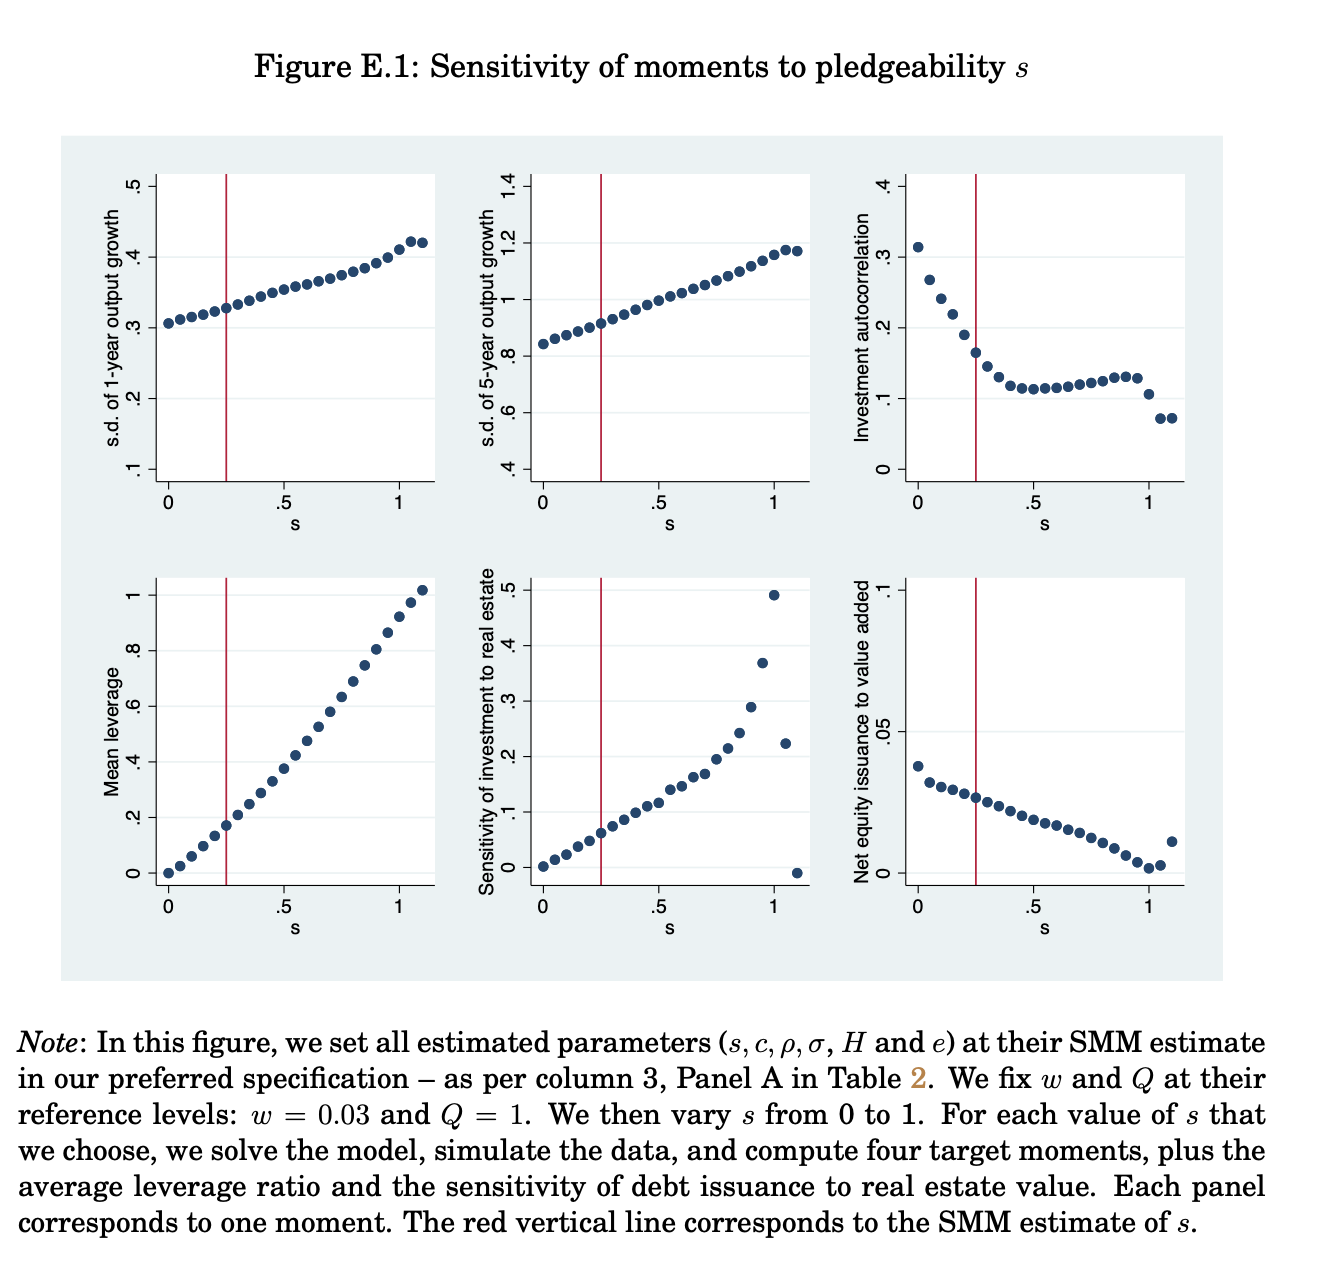
\includegraphics[scale=0.35]{figures/cchst_1}
\end{figure}
\end{frame}

\begin{frame}{Capital or Financial frictions?}
\begin{figure}
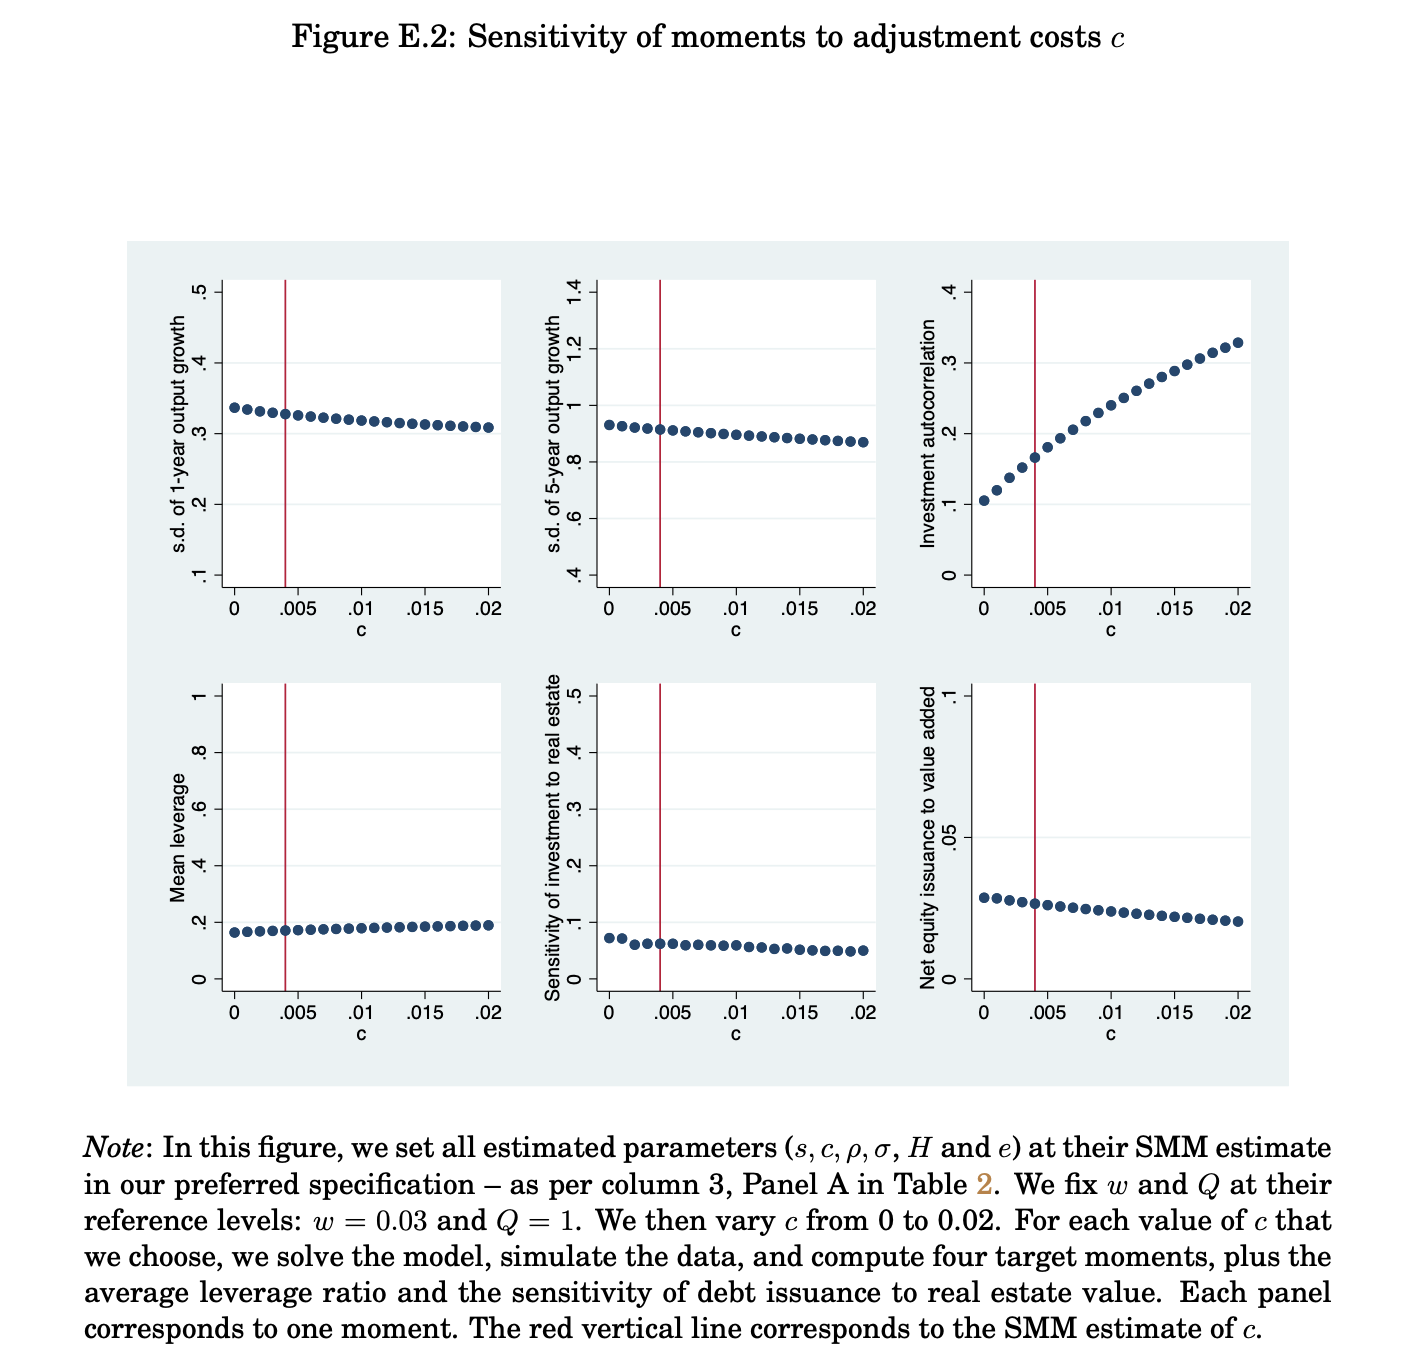
\includegraphics[scale=0.35]{figures/cchst_2}
\end{figure}
\end{frame}

\begin{frame}{GE Block}
\begin{itemize}
\item Aggregate production $Q$ is CES
\item Resource constraint
\[Q_t = C_t + I_t + AC_t\]
\item Quasi linear utility
\[L^s_t = \bar{L} w^{\epsilon}_t\] 
\end{itemize}
\end{frame}

\begin{frame}{Counterfactual}
\begin{itemize}
\item Two alternatives of creating the world with no financial constraints
\begin{enumerate}
\item $s \rightarrow \infty$
\item $e = 0$
\end{enumerate}
\item Which is the correct one?
\end{itemize}
\end{frame}

\begin{frame}{Results}
\begin{figure}
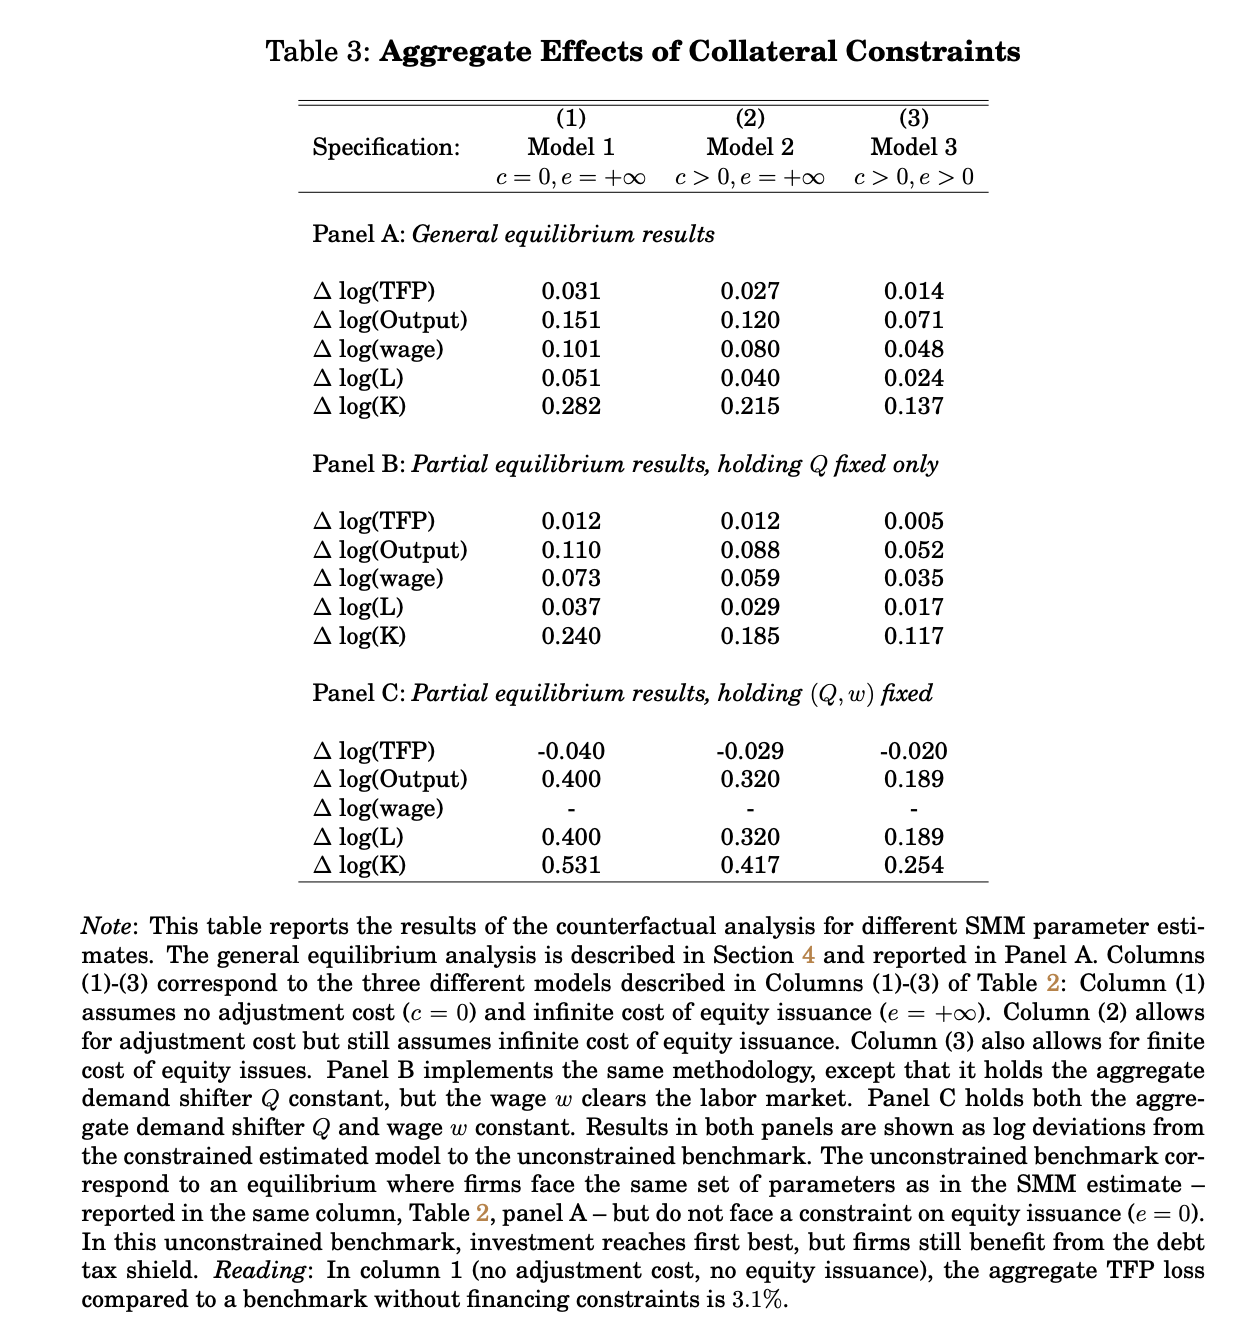
\includegraphics[scale=0.35]{figures/cchst_3}
\end{figure}
\end{frame}

\begin{frame}{Results}
\begin{itemize}
\item The results depend a lot on the persistence of productivity $\rho$
\item Why?
\item Recommended reading: Moll (2014)
\end{itemize}
\end{frame}

\begin{frame}{Mispecification}
\begin{itemize}
\item Two alternatives to estimate the model
\begin{itemize}
\item Estimate the structural parameters $\Theta$ to target (among others) $\beta$
\item Estimate the structural parameters $\Theta$ to target (among others) debt to capital ratios
\end{itemize}
\item Which is better?
\item Offer one metric: Effects of model mispecification
\item Also: Effect of measurement error
\end{itemize}
\end{frame}

\begin{frame}{Mispecification}
\begin{itemize}
\item Idea: Complicate the model
\begin{enumerate}
\item Intangible capital
\item Mismeasured capital
\item Economic depreciation $\neq$ accounting depreciation
\item Secured debt
\end{enumerate}
\item Estimate the extended and restricted (benchmark) model
\item What is the effect on the counterfactuals of TFP and output
\item Follows Isaiah, Gentzkow, Shapiro (2017) (which I should study).
\end{itemize}
\end{frame}

\begin{frame}{Mispecification}
\begin{figure}
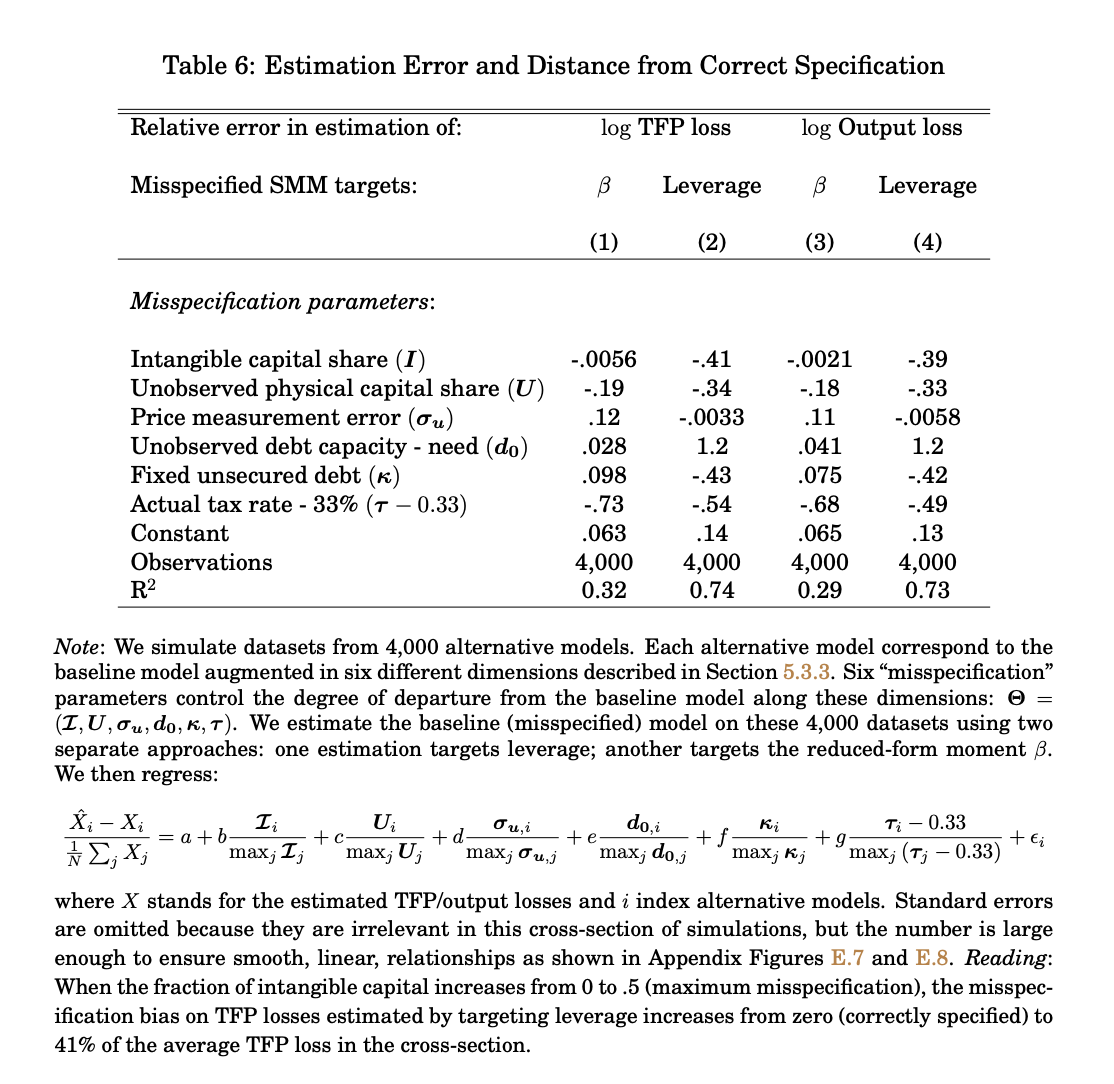
\includegraphics[scale=0.35]{figures/cchst_4}
\end{figure}
\end{frame}

\section{Bierdel, Drenik, Herre\~no, Ottonello (2021)}


\begin{frame}{Introduction}

\begin{itemize}
\item {\color{dblue}{Economic theories}}: asymmetric information plays central role in asset markets \smallskip
\begin{itemize}
\item affects quality, valuation, and liquidity of assets traded \\ \smallskip
 {\scriptsize{Akerlof 1970, Stiglitz Weiss 1981, Guerrieri Shimer Wright 2010}} \bigskip
\end{itemize} 

%\item Economies differ in  market development and info available to market participants \bigskip

\item How asymmetric information affects {\color{dred}{capital accumulation}}? \smallskip
\begin{itemize}
\item To what extent the quality of technologies that allow mkts participants to obtain info on capital quality can affect investment and income levels?
\end{itemize} 
\bigskip

\item {\color{dblue}{This paper}}:  Revisit these questions by combining \smallskip
\begin{itemize}
\item Capital-accumulation model with asymmetric information  \smallskip
\item Microlevel data informing the degree of information frictions

\end{itemize}

\end{itemize}

\end{frame}





%%%%%%%%%%%%%%%%%%%%%%%%%%%%%%%%%%%%%%%%%%%%%%%%%%%%%%%%%%%

\begin{frame}{Neoclassical Block}

\begin{itemize}

    \item {\color{dblue}{\bf Households}} \medskip
    \begin{itemize}

    \item Preferences $\mathbb E_{0}\sum \limits_{t=0}^{\infty} \beta^{t} u(c_{t})\gamma^t_{n}$
 \medskip

    \item  Endowed with $\bar{h}$ hours of work each period \medskip

    \item Access to a linear technology to produce new capital goods using final goods

\end{itemize}

\bigskip

\item {\color{dblue}{\bf  Firms }} \medskip

\begin{itemize}
\item Technology $y_{jt}=f_{t}(\mathcal K_{jt}, l_{jt})\equiv\mathcal K_{jt}^\alpha (\gamma^t l_{jt})^{1-\alpha}$  \medskip

\item With i.i.d. probability $\varphi$ firms exit the economy  \medskip

\item A new mass $\varphi$ of firms enter the economy

\end{itemize}
\end{itemize}

\end{frame}

\begin{frame}{Neoclassical Block}

\begin{itemize}

    \item {\color{dblue}{\bf Households}} $\Rightarrow$ hold unemployed capital, {\color{dred}{capital seller}} \medskip
    \begin{itemize}

    \item Preferences $\mathbb E_{0}\sum \limits_{t=0}^{\infty} \beta^{t} u(c_{t})\gamma^t_{n}$
 \medskip

    \item  Endowed with $\bar{h}$ hours of work each period \medskip

    \item Access to a linear technology to produce new capital goods using final goods

\end{itemize}

\bigskip

\item {\color{dblue}{\bf  Firms }} $\Rightarrow$ hold employed capital, {\color{dred}{capital buyer}} \medskip

\begin{itemize}
\item Technology $y_{jt}=f_{t}(\mathcal K_{jt}, l_{jt})\equiv\mathcal K_{jt}^\alpha (\gamma^t l_{jt})^{1-\alpha}$  \medskip

\item With i.i.d. probability $\varphi$ firms exit the economy  \medskip

\item A new mass $\varphi$ of firms enter the economy

\end{itemize}
\end{itemize}

\end{frame}

\begin{frame}{Capital-quality heterogeneity}

\begin{itemize}
\item  Capital stock composed of infinitesimal indivisible units  \medskip
%\begin{itemize}
%\item Available to trade in integer quantities only, and agents hold a mass of these units
%\end{itemize} \medskip

\item Capital units are heterogeneous in two dimensions \medskip

   \begin{itemize}
    \item {\color{dblue}{observed}} quality $\omega\in\Omega \equiv \left[\omega_1,\ldots,\omega_{N_\omega}\right]$ \medskip
    \item {\color{dred}{unobserved}} quality $a\in\mathcal{A}\equiv \left[a_1,\ldots,a_{N_a}\right]$\smallskip
    \begin{itemize}
    \item private information of owner
\end{itemize}
    \end{itemize}
    \medskip
    \item Capital services \smallskip
    \begin{itemize}
   \item  unit $i$: $\omega_{i} a_{i}$ \smallskip
    \item firm $j$'s capital input: $\mathcal K_{jt} ={\sum_{\omega  \in \Omega }} {\sum_{ a  \in \mathcal A}} \omega a k_{jt+1}(\omega, a)$
    \end{itemize}
 %   \medskip
%    \item Share of qualities in new capital governed by  $g: \Omega \times \mathcal A \rightarrow [0,1]$
\end{itemize}

\end{frame}

%%%%%%%%%%%%%%%%%%%%%%%%%%%%%%%%%

\begin{frame}{Decentralized Capital Market}

\begin{itemize}

\item Capital goods traded in a decentralized mkt with {\color{dblue}{\bf search-and-matching frictions}} \smallskip

\begin{itemize}

\item Consistent with microlevel evidence {\scriptsize{(Ramey Shapiro 2001, Gavazza 2011, Ottonello 2015)}}

\end{itemize} \medskip


%\item Based on empirical evidence trade in capital mkts (Gavazza 2011, Ottonello 2015) \medskip

\item Organized in a continuum of {\color{dred}{submarkets}}, indexed by ${\color{dred}{\boldsymbol {(\omega, \hat a, q)}}}\in \Omega \times \mathcal A \times \mathbb R_{+} $ \medskip

\item Search is {\color{dred}{directed}} {\scriptsize{(Shimer 1996, Moen 1997, Menzio Shi 2011)}} \smallskip

\begin{itemize}

\item Sellers list price $q(\omega,a)$ and announced quality $\hat{a}(\omega,a)$ \smallskip

\item Buyers dedicate hours of work to search and match $v_{t}(\omega, \hat a, q)$ \medskip

\end{itemize}

\item CRS matching technology in each submarket %$\mathcal M_{t}(k\Search_{t}(\omega, \hat a, q),v_{t}(\omega, \hat a, q))$
\medskip

\item Tightness $\theta _{t}(\omega, \hat a, q)\equiv \frac{v_{t}(\omega, \hat a, q)}{k\Search_{t}(\omega, \hat a, q)}$ \medskip

\item Sellers' matching probability $p(\theta_{t}(.))$, buyers' matching yield/hour $\mu_{t}(\theta_{t}(.))$
\end{itemize}

\end{frame}

\begin{frame}{Degree of Asymmetric information}\label{main:insp_protocol}

\begin{itemize}

\item Buyers have access to {\color{dblue}{\bf inspection technology}} {\scriptsize{(similar to Menzio Shi 2011)}} \smallskip
\begin{itemize}
\item prob $\psi$: that the buyer learns the true type $(\omega, a)$ of the capital good \smallskip
\item prob $1-\psi$: inspection is uninformative \smallskip
\end{itemize}
$\psi$ parameterizes the {\color{dred}{degree of asymmetric information}} in the economy
\bigskip
\item {\color{dblue}{\bf Trading protocol upon inspection}} \smallskip
\begin{itemize}
\item If no new info is revealed or capital quality is not below that announced (i.e., $a'\geq \hat a$) $\Rightarrow$ trade at price $q$  \medskip
\item If quality is some $a'<\hat a$: $\Rightarrow$ trade at $q^P_{t}(\omega,a',q)=\min\{\text{bargain price}, q\}$ \\(if there are gains from trade, no trade otherwise) 
\end{itemize}

%\item Buyers' beliefs $\pi_{a,t}(\omega,\hat{a}, q):\mathcal A^2 \times \mathbb{R}_{+}\rightarrow [0,1]$ \medskip

\end{itemize}


\end{frame}

\begin{frame}{Households' Capital Accumulation}

\bigskip
\begin{itemize}

\item Law of motion households' {\color{dblue}unemployed capital} of type $(\omega,a)$
\begin{align*}
k_{Ht+1}(\omega,a) =(1-p(\theta _{Ht} (\omega,a)))k_{Ht}(\omega,a)+g(\omega,a)i_{t}+\varphi K_{Ft}(\omega,a)
\end{align*}
\medskip
{\scriptsize{where $\theta _{Ht}(\omega,a)\equiv \theta _{t} (\omega,\hat{a}_{Ht}(\omega, a), {q}_{Ht}(\omega, a))$}}

\bigskip 

\item Euler equation for {\color{dblue} investment}
\begin{align*}
1={\sum_{\omega  \in \Omega }} {\sum_{ a  \in \mathcal A}}  g(\omega, a)\lambda_{t}({\mathbf{k}})\nu\Seller_{t+1}(\omega,a,\mathbf{k}),
\end{align*}
Q-Theory Interpretation, allowing for heterogeneity, search, and AI
\end{itemize}
\medskip

\end{frame}

\begin{frame}{Households as Capital Sellers}

\begin{itemize}

\item {\color{dblue} Marginal value of capital}
\begin{align*}
\nu^{\mathrm{s}}_{t}(\omega,a,\mathbf{k}) =\max_{ \hat a, q} \:\: & p(\theta_t(\omega,\hat a, {q}))((1-\psi)q + \psi q^{P}_{t}(\omega,a,q)) \notag\\
&+ \left(1-  p(\theta_t(\omega,\hat a,{q}))\right) (\lambda_{t}({\mathbf{k}}) \nu^{\mathrm{s}}_{t+1}(\omega,a,k_{Ht}(\mathbf{k})) - \delta \omega a)
\end{align*}

\begin{figure}
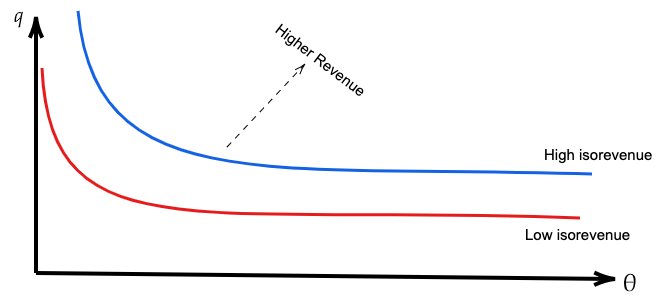
\includegraphics[scale=0.4]{figures/isorevenues_new.png}
\end{figure}
\end{itemize}

\end{frame}







\begin{frame}{Firms' Capital Accumulation}

\begin{itemize}

\item Law of motion firms' {\color{dblue}employed capital} of type $(\omega,a)$
\begin{align*}
k_{jt+1}(\omega,a) =\sum_{\hat a} \int_{q \in \mathbb{R}_{+}}\iota_{t}(a|\omega,\hat{a},q)\mu_{t}\left(\theta_{t}\left(\omega,\hat a,q\right)\right)v_{jt}(\omega,\hat a,q) \diff q+k_{jt}(\omega,a)
\end{align*}
\medskip
{\scriptsize{where $\iota_{t}(a|\omega,\hat{a},q)$: share of capital quality $a$ in submarket $(\omega,\hat{a}, q)$ }}
\bigskip
\item {\color{dblue} Marginal value of capital}
\begin{align*}
\nu^{\mathrm{b}}_{t}(\omega,a) &= (Z_t - \delta) \omega a  +  \Lambda_{t,t+1} \left[ (1-\varphi) \nu^{\mathrm{b}}_{t+1}(\omega,a) + \varphi \nu^{\mathrm{s}}_{t+1}(\omega,a,{\mathbf{K}}_{Ht}) \right],
\end{align*}
{\scriptsize{where $Z_t \equiv  \alpha \left( \frac{\gamma^t (1-\alpha)}{w_t}\right)^{\frac{1-\alpha}{\alpha}}$}}

\end{itemize}

\end{frame}

\begin{frame}{Firms as Capital Buyers}

\begin{itemize}

\item {\color{dblue}Optimal search activity across submarkets}
{\scriptsize
\begin{equation*}
{v}_{t}(\omega,\hat a, q)\left( \underbrace{((1-\psi)q + \psi \mathbb E_a(q^{P}_{t}(\omega,a,q)|\omega,\hat a,q))}_\text{Expected price}+ \underbrace{\frac{w_{t}}{\mu_{t}(\theta(\omega,\hat a,q))}}_\text{Search cost}-\underbrace{\mathbb E_a \left( \nu^{\mathrm{b}}_{t}(\omega,a)| \omega,\hat a,q\right) }_{\text{Expected value}}\right)^{+}=0,
\label{buyer_indifference}
\end{equation*}}

\begin{figure}
\scalebox{.6}{\import{figures/}{isocost_new.tex}}
\end{figure}


\end{itemize}


\end{frame}

%%%%%%%%%%%%%%%%%%
\begin{frame}{Equilibrium Under Full Information}

\begin{itemize}

\item Suppose $\Omega=\{{\color{red}{\omega_L}},{\color{blue}{\omega_H}}\}$, $\mathcal{A}=\{\overline{a}\}$
\bigskip

\begin{figure}
\scalebox{.75}{\import{figures/}{eq_fi.tex}}
\end{figure}


\end{itemize}

\end{frame}
%%%%%%%%%%%%%%%%%%


\begin{frame}{Prices and Duration Under Full Information}\label{main:full_info}

Prediction I: Under FI there is a  {\color{dblue}{\bf negative relationship between prices and duration}} \medskip

$q\FullInfo(\omega_{H},a)>q\FullInfo(\omega_{L},a), p\left(\theta\FullInfo(\omega_{H},a)\right)>p\left(\theta\FullInfo(\omega_{L},a)\right)$ \medskip


\bigskip

{{\color{dblue}{Intuition}}: Submarkets with higher quality attract more buyers resulting on higher prices and lower matching probability for buyers
%\vspace{-0.2cm}
\begin{align*}\small
\underbrace{(1-\eta)\left(\nu\Buyer(\omega,a)-\beta \nu\Seller(\omega,a) \right)}_{\text{benefit purchasing quality $(\omega,a)$}}= \underbrace{\frac{\theta(\omega,a)\chi}{p\left(\theta(\omega,a)\right)}}_{\text{search cost}}
\end{align*}
}


\end{frame}



%%%%%%%%%%%%%%%%%%
\begin{frame}{Equilibrium Under Asymmetric Information}

\begin{itemize}

\bigskip

\item Suppose $\mathcal A=\{a_L,a_H\}$
\bigskip

\item Consider PBE under intuitive criterion  ({\small{Cho Kreps 1987}})  
\begin{itemize}
\item fully-revealing separating and pooling equilibria 
\end{itemize}

\medskip

\item Focus on balanced-growth path  \bigskip

\item Results extend to multiple types and transitional dynamics

\end{itemize}

\end{frame}
%%%%%%%%%%%%%%%%%%

%%%%%%%%%%%%%%%%%%
\begin{frame}{Constructing the Equilibrium}

\begin{itemize}

\item For {\color{dred}{\bf low type}}
{\small\begin{align*}
\nu^{\mathrm{s}}(\omega,a_{L}) & = \max_{\{ q(\omega, a_{L})\}} p\left(\theta\left(\omega,a_{L},{q}(\omega, a_{L})\right)\right)  q(\omega,a_{L})    \\ \notag
&+ \left(1-  p(\theta(\omega,a_{L},{q}(\omega, a_{L})))\right) \left(\beta \nu^{\mathrm{s}}(\omega,a_{L}) - \delta \omega a_{L}\right)\\
\text{subject to}\\
\theta(\omega,a_{L},&q(\omega,a_{L})) = \mu^{-1} \left( \frac{w}{\nu\Buyer(\omega,a_{L})   - q(\omega,a_{L})} \right)
\end{align*}}


\end{itemize}

\end{frame}
%%%%%%%%%%%%%%%%%%


%%%%%%%%%%%%%%%%%%
\begin{frame}{Constructing the Equilibrium}

\begin{itemize}

\item For low type \medskip

\item For {\color{dblue}{\bf high type}}:
{\small\begin{align*}
\nu^{\mathrm{s}}(\omega,a_{H}) & = \max_{\{ q(\omega, a_{H})\}} p\left(\theta\left(\omega,a_{H},{q}(\omega, a_{H})\right)\right)  q(\omega,a_{H})    \\ \notag
&+ \left(1-  p(\theta(\omega,a_{H},{q}(\omega, a_{H})))\right) \left(\beta \nu^{\mathrm{s}}(\omega,a_{H}) - \delta \omega a_{H}\right)\\
\text{subject to}\\
\theta(\omega,a_{H},&q(\omega,a_{H})) = \mu^{-1} \left( \frac{w}{\nu\Buyer(\omega,a_{H})   - q(\omega,a_{H})} \right),\\
\\ \notag
\nu^{\mathrm{s}}(\omega,a_{L}) & \geq p\left(\theta\left(\omega,a_{H},{q}(\omega, a_{H})\right)\right) \left((1-\psi) q(\omega,a_{H}) + \psi q^P_{t}(\omega,a_{L},{q}(\omega, a_{H}))\right) \\ \notag
&+ \left(1-  p(\theta(\omega,a_{H},{q}(\omega, a_{H})))\right) \left(\beta \nu^{\mathrm{s}}(\omega,a_{L}) - \delta \omega a_{L}\right)
\end{align*}} 
\item {\color{dblue}{Proposition}}: There exists a unique fully-revealing separating equilibrium that satisfies the intuitive criterion; there are no pooling equilibria \bigskip
\end{itemize}

\end{frame}
%%%%%%%%%%%%%%%%%%


%%%%%%%%%%%%%%%%%%


\begin{frame}{Equilibrium Under Asymmetric Information}
\begin{figure}
\scalebox{.75}{\import{./Figures/}{eq_fi.tex}}
\end{figure}
\end{frame}


\begin{frame}{Equilibrium Under Asymmetric Information}
\begin{figure}
\scalebox{.75}{\import{./Figures/}{no_mimicking_1.tex}}
\end{figure}
\end{frame}

\begin{frame}{Equilibrium Under Asymmetric Information}
\begin{figure}
\scalebox{.75}{\import{./Figures/}{no_mimicking_2.tex}}
\end{figure}
\end{frame}

\begin{frame}{Equilibrium Under Asymmetric Information}
\begin{figure}
\scalebox{.75}{\import{./Figures/}{no_mimicking_3.tex}}
\end{figure}
\end{frame}

%%%%%%%%%%%%%%%%%%

%%%%%%%%%%%%%%%%%%
\begin{frame}{Equilibrium Under Asymmetric Information}
\scalebox{.75}{\import{./Figures/}{p_q_phi.tex}}
\end{frame}
%%%%%%%%%%%%%%%%%%


\begin{frame}{Prices and Duration Asymmetric Information}\label{main:asym_info}

Prediction II: \\

{\color{dred}{\bf AI}} (i.e., $\psi<\psi^*$) affects {\color{dblue}{terms of trade of high-quality capital}} \\ \smallskip

$q(\omega,a_{H})>q^{FI}(\omega,a_{H}), p\left(\theta(\omega,a_{H})\right)<p\left(\theta^{FI}(\omega,a_{H})\right)$
\bigskip


\begin{itemize}
\item {\color{dblue}Intuition}: $a_H$ chooses higher price to signal its quality, willing to accept lower trading probability \medskip
\item Distortions governed by $\psi$: $\frac{ d\left[ln \frac{p(\theta(\omega,a_L))}{p(\theta(\omega,a_H)) } \right] }{d\psi}\Big|_{\psi < \psi^*} < 0$\medskip
\item {\bf{\color{dblue}{Relationship between prices and duration is informative about $\psi$}}}
\end{itemize}

\end{frame}









%%%%%%%%%%%%%%%%%%%%%%%%%%%%%%%%%%%%%%%%%%%%%%%%%%%%%%%%%%%%%%%%%%%%%%%%%%%%%%%%%
%%%%%%%%%%%%%%%%%%%%%%%%%%%%%%%%%%%%%%%%%%%%%%%%%%%%%%%%%%%%%%%%%%%%%%%%%%%%%%%%%

\begin{frame}[label=thedata]{The Data}

\begin{itemize}

\item Panel of {\color{dred}{capital structures}} posted for sale and rent  \smallskip
\begin{itemize}
\item Retail, office space, and warehouses \smallskip
\item Monthly listed price \smallskip
\item Contain information on listed characteristics: \\ location, age, size, number of rooms, etc \smallskip
\item Duration and monthly search intensity (clicks and emails)
\end{itemize}\bigskip


\item {\color{dblue}{Source}}: \textit{Idealista}, leading online platform in the real estate market in Europe \bigskip

\item {\color{dblue}{Coverage}}: 8.5 million observations from Spain \smallskip
\begin{itemize}
\item $>$ 1.1 million capital units \smallskip
\item Period: 2005--2018
\end{itemize}

\end{itemize}


\end{frame}

%%%%%%%%%%%%%%%%%%%%%%%%%%%%%%%%%%%%%%%%%%%%%%%%%%%%%%%%%%%%%%%%%%%%%%%%%%%%%%%%%


%%%%%%%%%%%%%%%%%%%%%%%%%%%%%%%%%%%%%%%%%%%%%%%%%%%%%%%%%%%%%%%%%%%%%%%%%%%%%%%%%

\begin{frame}{Price Variation Explained by Listed Characteristics}
\medskip
\begin{center}
{(Log) price per sq. ft. of property $i$ in location $l$ in month $t$:}
$$log(q_{ilt}) = \nu_{lt} + \gamma X_{i} + \varepsilon_{ilt}$$
\end{center}
\begin{minipage}{.5\textwidth}
\begin{table}
\begin{tabularx}{5.9cm}{lcc}
\toprule
{}&{Std. Sale}&{R sq. Sale} \tabularnewline
\midrule \addlinespace[\belowrulesep]
Raw data&0.75&0.00 \tabularnewline
\midrule Year &0.71&0.12 \tabularnewline
Location&0.54&0.48 \tabularnewline
Year x Loc&0.49&0.57 \tabularnewline
... x Type&0.48&0.59 \tabularnewline
... x Area&0.38&0.74 \tabularnewline
... x Age&0.37&0.75 \tabularnewline
\midrule
Benchmark&0.37&0.75 \tabularnewline
\bottomrule
\end{tabularx}
\end{table}
\end{minipage}
\begin{minipage}{.3\textwidth}
\begin{figure}[H]
\centering
\includegraphics[scale=0.24]{figures/hist_satur_2.png}
% \caption{Raw and Residual Prices - Saturated - Sale}
\end{figure}
\end{minipage}
\end{frame}


%%%%%%%%%%%%%%%%%%%%%%%%%%%%%%%%%%%%%%%%%%%%%%%%%%%%%%%%%%%%%%%%%%%%%%%%%%%%%%%%%
%
%\begin{frame}{Price Dispersion: Sales}
%\begin{figure}[H]
%\centering
%\includegraphics[width=0.6\textwidth]{../../Draft/facts_paper/Draft_11/Figures/hist_satur_2.png}
%% \caption{Raw and Residual Prices - Saturated - Sale}
%\end{figure}
%\end{frame}

%%%%%%%%%%%%%%%%%%%%%%%%%%%%%%%%%%%%%%%%%%%%%%%%%%%%%%%%%%%%%%%%%%%%%%%%%%%%%%%%%
%%%%%%%%%%%%%%%%%%%%%%%%%%%%%%%%%%%%%%%%%%%%%%%%%%%%%%%%%%%%%%%%%%%%%%%%%%%%%%%%%

\begin{frame}{Duration and Prices}

\begin{minipage}{.45\textwidth}
\begin{table}
\scriptsize
\begin{tabular}{c}
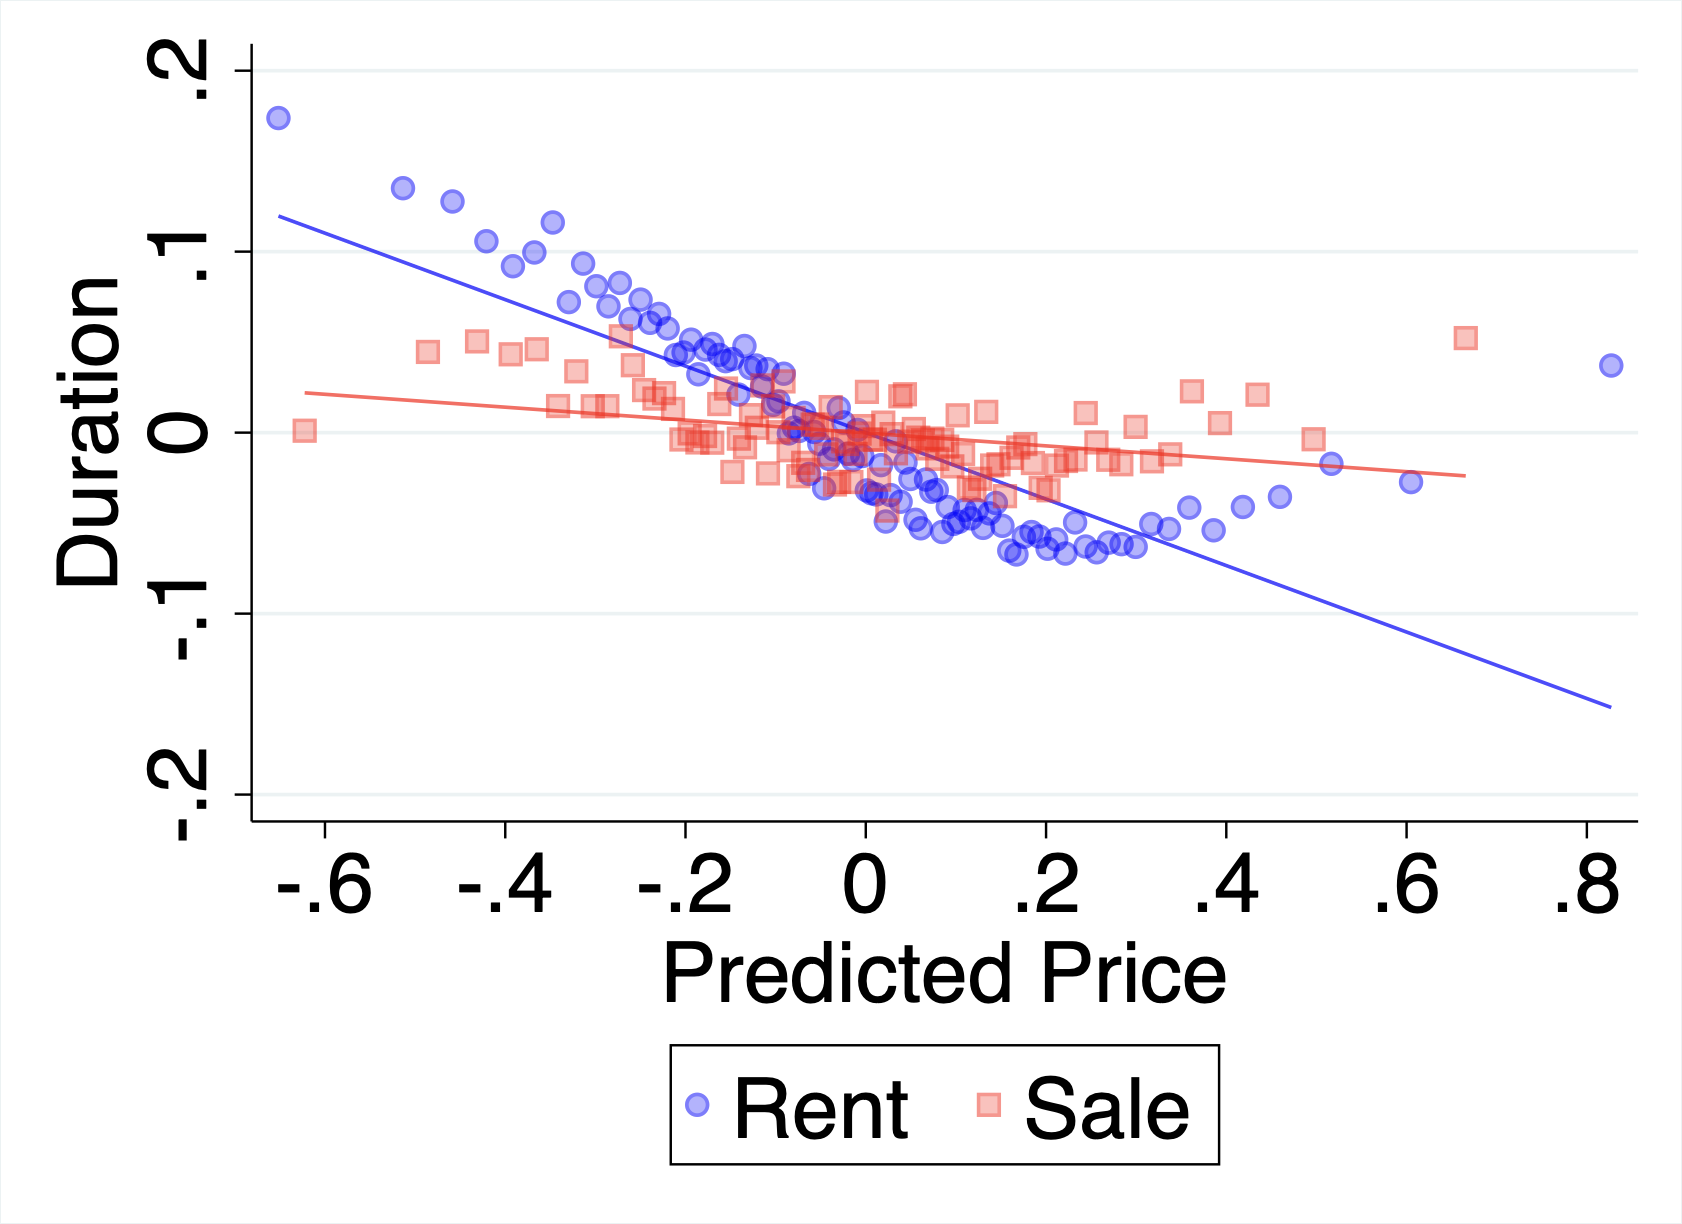
\includegraphics[scale = 0.22]{figures/binscatter_pred_dur_rent_sale.png}
\end{tabular}
% \caption{Predicted and Residual Price by Operation Type}
\end{table}
\end{minipage}
\begin{minipage}{.45\textwidth}
\begin{table}
\scriptsize
\begin{tabular}{c}
\includegraphics[scale = 0.22]{figures/binscatter_pres_dur_rent_sale.png}
\end{tabular}
% \caption{Predicted and Residual Price by Operation Type}
\end{table}
\end{minipage}
\begin{itemize}
\item Consistent with model predictions under FI and AI
\end{itemize}
\end{frame}

%%%%%%%%%%%%%%%%%%%%%%%%%%%%%%%%%%%%%%%%%%%%%%%%%%%%%%%%%%%%%%%%%%%%%%%%%%%%%%%%%
%%%%%%%%%%%%%%%%%%%%%%%%%%%%%%%%%%%%%%%%%%%%%%%%%%%%%%%%%%%%%%%%%%%%%%%%%%%%%%%%%

%\begin{frame}[noframenumbering]{Duration and Residual Prices}
%
%\begin{table}
%\scriptsize
%\begin{tabular}{c}
%\includegraphics[width=0.6\textwidth]{../../Draft/facts_paper/Draft_11/Figures/binscatter_pres_dur_rent_sale.png}
%\end{tabular}
%% \caption{Predicted and Residual Price by Operation Type}
%\end{table}
%\vspace{-0.5cm}
%\begin{itemize}
%\item Consistent with the presence of Asymmetric Information
%\end{itemize}
%
%\end{frame}

%%%%%%%%%%%%%%%%%%%%%%%%%%%%%%%%%%%%%%%%%%%%%%%%%%%%%%%%%%%%%%%%%%%%%%%%%%%%%%%%%
%%%%%%%%%%%%%%%%%%%%%%%%%%%%%%%%%%%%%%%%%%%%%%%%%%%%%%%%%%%%%%%%%%%%%%%%%%%%%%%%%

\begin{frame}[label=pricesduration]{Prices and Duration}



\begin{table}
\scriptsize
% \caption{Predicted and Residual Price by Operation Type}
{
\begin{tabular}{l*{4}{c}}
\hline\hline
                              &\multicolumn{1}{c}{(1)}&\multicolumn{1}{c}{(2)}\\
                              &\multicolumn{1}{c}{$\log$ Dur}&\multicolumn{1}{c}{$\log$ Dur}\\
\hline
log price                     &     0.013***&            \\
                              &   (0.002)   &             \\
Predicted Price               &             &    -0.018*   \\
                              &             &   (0.010)    \\
Residual Price                &             &     0.154***&  \\
                              &             &   (0.004)   &   \\
Constant                      &     1.961***&     2.108***\\
                              &   (0.008)   &   (0.046)      \\
\hline
Observations                  &    456,351   &    439,680   \\
\(R^{2}\)                     &     0.000   &     0.202     \\
Subsample                    &      Sale   &      Sale   \\
Fixed Effects                 &        No   &       Yes    \\
\hline\hline
\end{tabular}
}
\end{table}
\begin{itemize}
\item Results robust to other measures of search behavior 
\end{itemize}
\end{frame}

%%%%%%%%%%%%%%%%%%%%%%%%%%%%%%%%%%%%%%%%%%%%%%%%%%%%%%%%%%%%%%%%%%%%%%%%%%%%%%%%%
%%%%%%%%%%%%%%%%%%%%%%%%%%%%%%%%%%%%%%%%%%%%%%%%%%%%%%%%%%%%%%%%%%%%%%%%%%%%%%%%%

\begin{frame}{Alternative Explanations}

\begin{enumerate}
\item Sellers' indifference between price and duration
\begin{itemize}
\item Expected revenues higher for higher residual prices \smallskip
\item Even for impatient and risk averse sellers
\end{itemize} \medskip
\item Heterogeneity in sellers' preferences \smallskip
\begin{itemize}
\item Discounting and risk aversion
% \item Under FI, heterogeneity in $\beta$ pushes slope upwards\smallskip
% \item Slope remains negative in locations with higher firm exit rates
\end{itemize} \medskip
\item Heterogeneity in sellers' holding costs 
\begin{itemize}
\item To rationalize choices, holding costs must be extremely large
\end{itemize}
\end{enumerate}

\end{frame}


%%%%%%%%%%%%%%%%%%

\begin{frame}{Parameterization}

{\color{dblue}{Two-step procedure}}
\begin{enumerate}
\item {\bf{Fix a subset of parameters to standard values}}
\item {\color{gray}{Calibrate targeting moments on model simulated data}}
\end{enumerate}
\bigskip
\begin{footnotesize}
\begin{table}
\begin{tabular}{llc}
\hline
\hline
{\bf{Parameter}} & {\bf{Description}} & {\bf{Value}}\\
\hline
$\beta$ & Discount factor & 0.9966 \\
$\alpha$ & Share of capital & 0.35 \\
$\gamma$ & Technology growth & 1.004 \\
$\gamma_n$ & Population growth & 1.0027 \\
$\varphi$ & Firms' exit rate & 0.0027 \\
$\phi$ & Bargaining power of sellers & 0.5\\
$\eta$ & Curvature matching technology & 0.8 \\
\hline
\hline
\end{tabular}
\end{table}
\end{footnotesize}
\end{frame}



\begin{frame}{Parameterization}

{\color{dblue}{Two-step procedure}}
\begin{enumerate}
\item {\color{gray}{Fix a subset of parameters to standard values}}
\item {\bf{Calibrate targeting moments on model simulated data}}
\end{enumerate}
\bigskip
\begin{footnotesize}
\begin{table}
\begin{tabular}{llc}
\hline
\hline
{\bf{Parameter}} & {\bf{Description}} & {\bf{Value}}\\
\hline
$\bar{m}$ & Efficiency matching technology & 1.55 \\
$\sigma_\omega$ & SD of observed capital quality & 0.65  \\
$\sigma_a$ & SD of unobserved quality & 0.61\\
$\psi$ & Accuracy inspection technology & 0.92 \\
\hline
\hline
\end{tabular}
\end{table}
\begin{table}
\begin{tabular}{lccc}
\hline
\hline
Moment & Data & Model \\
\hline
Mean duration & 7.55 & 8.04 \\
SD predicted prices &0.593  & 0.595  \\
SD residual prices & 0.546 &  0.563  \\
slope $\log dur$ and residual prices & 0.154 & 0.153 \\ \hline \hline
%\hline
\end{tabular}
\end{table}
\end{footnotesize}
\end{frame}




\begin{frame}{Identification}
In the model, the extent of asymmetry of information $\psi$ is identified by the projection of $\log$
durations on $\log$ prices controlling for the observed component of capital quality. The variance of the distribution of unobserved qualities $\sigma^2_a$
is then identified by the variance of residual prices.
\end{frame}


%%%%%%%%%%%%%%%%%%%%%%%%%%%%%%%%%%%%%%%%

\begin{frame}{Effects of Asymmetric Informations on Capital Markets}
\begin{table}
\scriptsize
\begin{tabular}{c}
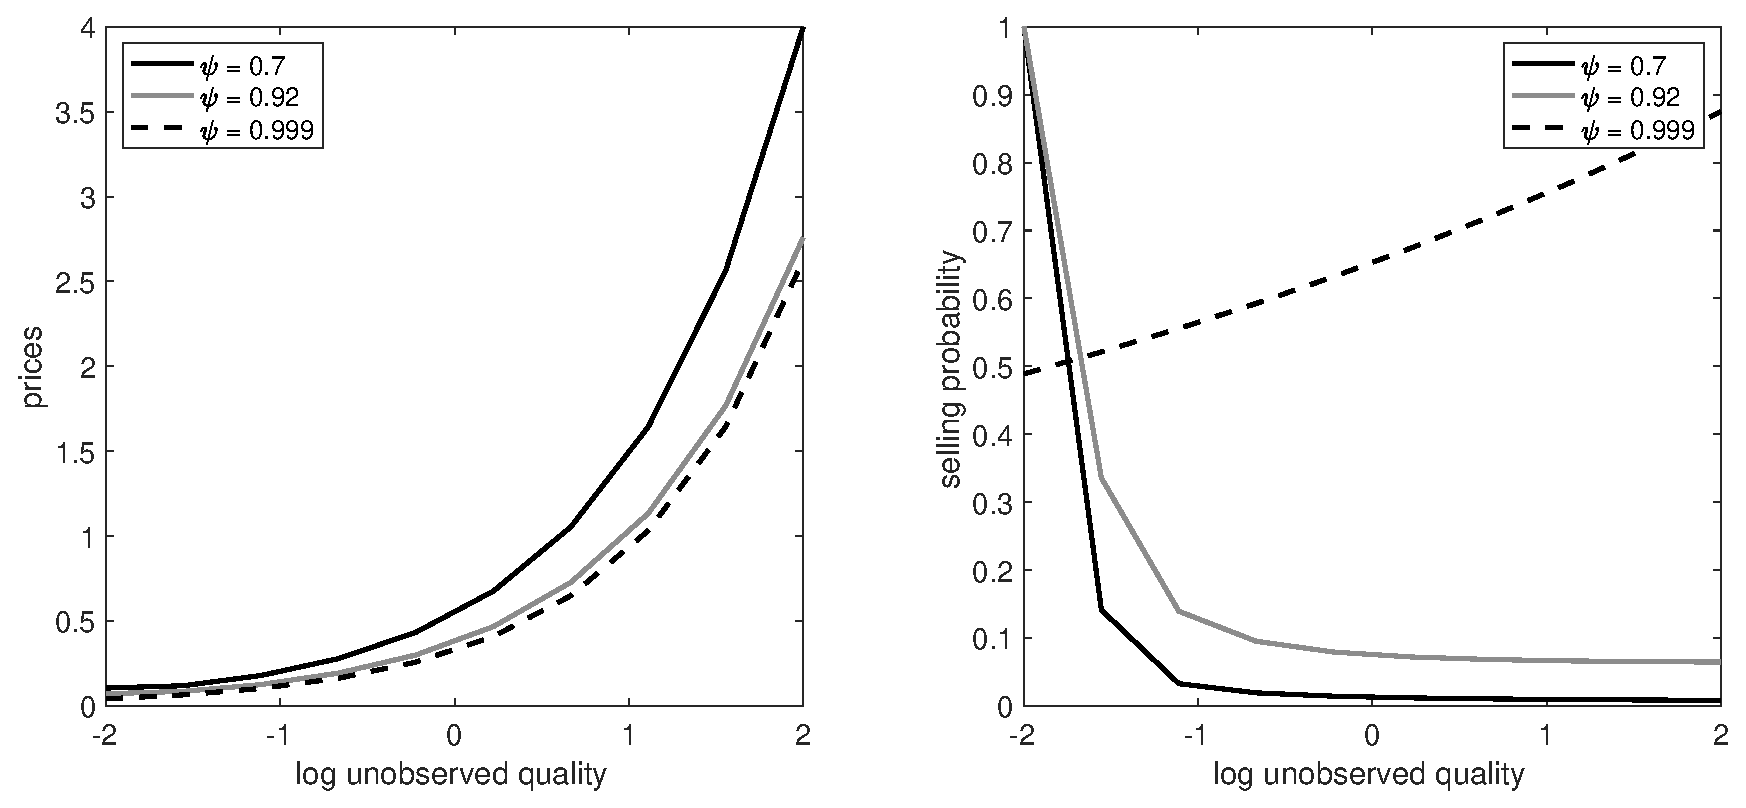
\includegraphics[width=0.9\textwidth]{figures/fig_policy_functions.eps}
\end{tabular}
% \caption{Predicted and Residual Price by Operation Type}
\end{table}
\vspace{-0.5cm}
\end{frame}

\begin{frame}{Macroeconomic Effects of Asymmetric Information}\label{app:macro_implications_ai}

\begin{itemize}
\item Aggregate output can be represented by
\end{itemize}

{\footnotesize\begin{equation*}
Y_t = \left(\gamma^t L_t\right)^{1-\alpha}\left(\underbrace{\left[\sum_{\omega\in\omega}\sum_{a\in\mathcal{A}}K_{t}(\omega,a)\right]}_{\text{capital stock}}\left[\mathbb{E}\left(\omega a\right)\left(1-\underbrace{\mathbb{E}\left(u_{t}(\omega,a)\right)}_{\text{capital unemployment}}\right)-\underbrace{\mathbb{C}ov\left(\omega a,u_{t}(\omega,a)\right)}_{\text{quality of unemployed capital}}\right]\right)^{\alpha}
\end{equation*}}
\end{frame}


\begin{frame}{Macroeconomic Effects of Asymmetric Information}
\begin{table}
\scriptsize
\begin{tabular}{c}
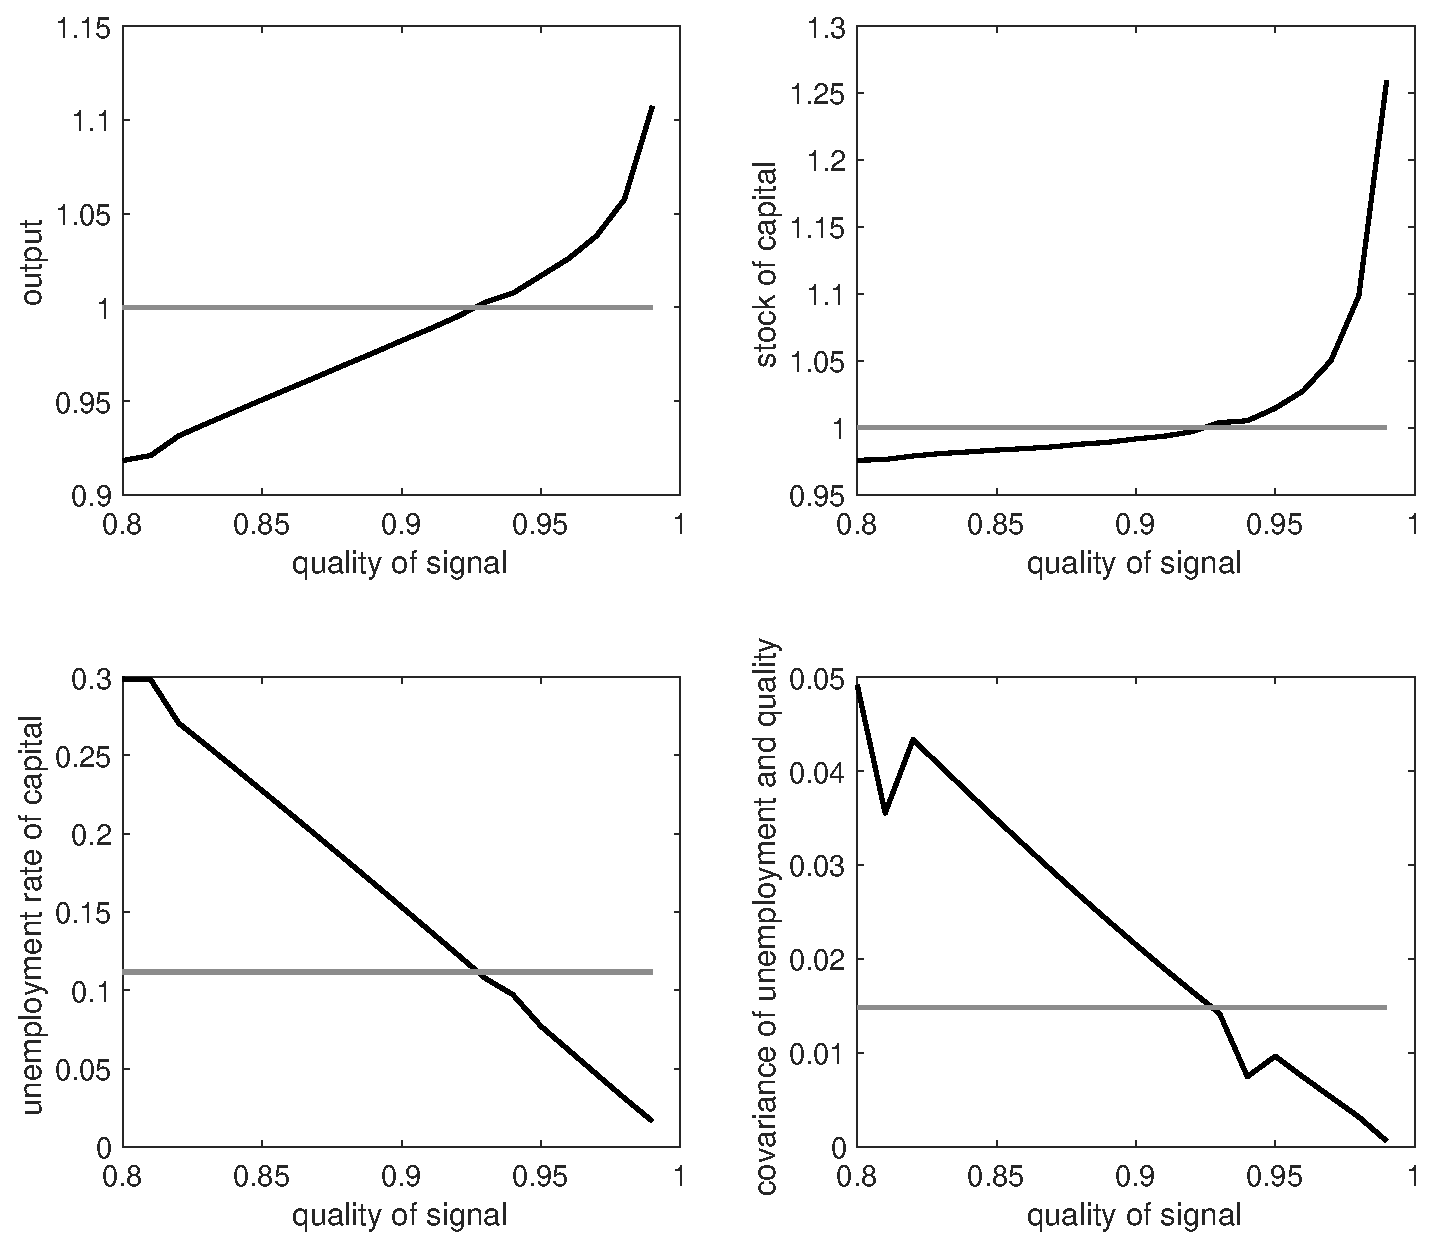
\includegraphics[width=0.6\textwidth]{figures/fig_macro}
\end{tabular}
% \caption{Predicted and Residual Price by Operation Type}
\end{table}
\vspace{-0.5cm}
\end{frame}

\begin{frame}{Macroeconomic Effects of Asymmetric Information:\\ Decomposition of Channels}
\begin{table}
\begin{tabular}{lc}
\hline
\hline
Variable & Value \\
\hline
Output effect of full information & 9.7\% \\
Investment channel  & 6.5\% \\
Capital-unemployment channel & 2.8\% \\
Capital-quality channel &  0.2\% \\
\hline
\hline
\end{tabular}
\end{table}
\end{frame}



\begin{frame}{Conclusions}

\begin{itemize}

\item Information asymmetries in capital markets have important macroeconomic implications \smallskip
\begin{itemize}
\item Investment, misallocation, and long-run income levels
\end{itemize}
\bigskip
\item Results suggest importance of studying \medskip
\begin{itemize}
\item capital-market policies designed to address potential inefficiencies that arise from information asymmetries  \medskip
\item agents' incentives of developing data and information technologies that mitigate information frictions (e.g., Jones Tonetti 2020, Farboodi Veldkamp 2021)
\end{itemize}
\end{itemize}
\end{frame}

\section{Winberry (2021)}


\begin{frame}{Neoclassical Firms very sensitive to changes in the Real Interest Rate}
\begin{itemize}
\item Time is discrete time, each period is a year.
\item Simplest determination of capital $\delta = 0$
$$A F_k = r $$
\item Assume that $F(K,L) = K^{\alpha}L^{1-\alpha}$. Therefore:
$$1+r_t = 1+ A_t \alpha K_t^{\alpha-1}L_t^{1-\alpha}$$
\vspace{-0.5cm}
\item Make a log-linear approximation. Hatted variables are log changes:
$$\hat{r}_t = \frac{r}{1+r}\left(\hat{a}_t - (1-\alpha) \hat{k}_t + (1-\alpha) \hat{l}_t\right)$$
\vspace{-0.5cm}
\item where $\hat{r_t} = \log \frac{1+r_t}{1+r}$
\end{itemize}
\end{frame}



\begin{frame}{Neoclassical Firms very sensitive to changes in the Real Interest Rate}
$$\hat{k}_t = - \hat{r}_t \left(\frac{1+r}{(1-\alpha)r}\right) + \frac{\hat{a}_t}{1-\alpha} + \hat{l}_t$$
\begin{itemize}
\item Assume an exogenous decrease of 1\% in interest rates.
\item Capital would have to increase 31.5\%  
\item Including reasonable depreciation would change this number to 14\%.
\item Letting labor increase would further increase this number
\item Assume 100\% of GDP could be transformed to capital.
\item Capital-output ratios are between 2 and 4 (depending on land and housing)
\item To increase capital by 31\%, it would take 61\%-124\% of GDP
\item With $\delta$: to increase capital by 14\%, it would take 28-56\% of GDP
\end{itemize}
\end{frame}


\begin{frame}{Another way of seeing the same}
\begin{itemize}
\item Another way of illustrating the same issue is to compute the semi-elasticity of investment to interest rates
\item Imagine firms with DRS
\[y_j = z \epsilon_j k_j^{\alpha}\]
\item Then
\[\frac{\partial i_{jt}/i_{jt}}{ \partial r_t} = - \frac{1}{\delta} \frac{1}{1-\alpha}\left(\frac{1+r_t}{r_t + \delta}\right) \]
\item As $\alpha \rightarrow 1$, the semi-elasticity becomes infinite
\item Under $\alpha = 0.7$, $\delta = 0.025$ $r_t = 0.01$
\item The semi-elasticity is equal to -3,847
\end{itemize}
\end{frame}


\begin{frame}{Capital Adjustment Frictions}
\begin{itemize}
\item Very large literature
\item 70s: Abel (1979)
\item 80s: Hayashi (1982)
\item 90s: Doms and Dunne (1998), Caballero (1999), Caballero and Engel (1999)
\item 2000s: Thomas (2000), Cooper and Haltiwanger (2006), Khan and Thomas (2003, 2008), Gourio Kashyap (2007)
\item Just to name a few
\end{itemize}
\end{frame}

\begin{frame}{Some Context}
\begin{itemize}
\item Capital accumulation models tend to have adjustment costs
\item One reason is what we saw before
\item in CT: Without any costs, in a standard model investment functions are not well-defined
\item Convex Adjustment costs. Two main results:
\begin{enumerate}
\item Investment is a function of $q$: The marginal value of one extra unit of capital
\[\frac{i_{jt}}{k_{jt}} = h(q_t)\]
\item Marginal ($q$) and average ($Q$) values of capital are equal, when some conditions apply
\[q_t = Q_t\]
\end{enumerate}
\item Very tractable problem. Block in medium-scale DSGE models
\end{itemize}
\end{frame}

\begin{frame}{Some Context}
Issue:
\begin{itemize}
\item Evidence of lumpiness of investment at the individual level
\item Lumpy investment: Periods of inaction followed by spikes in investment
\item Obviously convex adjustment costs do not get that
\item Documented originally by Doms and Dunne (1998)
\item The literature proposed fixed costs of adjustment as a possible answer
\item Cooper and Haltiwanger (2006) interpret the microdata as exhibiting both convex and non-convex costs
\item For the purpose of our class: Does micro-level frictions of capital adjustment matter in the aggregate?
\end{itemize}
\end{frame}


\begin{frame}{Metric}
\begin{itemize}
\item What does it mean that micro frictions ``matter'' for the aggregate
\item Is the response to shocks the same in models with and without fixed costs
\item One particular dimension receives interest: Pent-up demand
\item Or in more technical jargon, state-dependence of the elasticity of investment to aggregate shocks
\item Is the response of investment to a TFP shock higher or lower in a recession?
\item RBC model: It's the same
\item Alternative: Pent-up demand, the elasticity depends on the distribution of capital imbalances
\item At the start of the recovery firms have ``excess capital'', so an additional shock may not trigger large adjustments
\end{itemize}
\end{frame}

\begin{frame}{Early findings}
\begin{itemize}
\item Response by Thomas (2002): No
\item Micro level lumpiness is irrelevant 
\item Meaning: Models with and without lumpiness as observed in the data have the same aggregate dynamics
\end{itemize}
\end{frame}





\begin{frame}{Winberry 2021}
$$\frac{\partial i_{jt}/i_{jt}}{\partial r_t} = - \frac{1}{1-\alpha}\frac{1}{\delta}\frac{1+r_t}{r_t + \delta}$$
\begin{itemize}
\item Under a reasonable calibration:
\item $\alpha = 0.7$, $\delta = 0.025$, $r_t = 0.01$: $\frac{\partial i_{jt}/i_{jt}}{\partial r_t} = -3,847$
\item $r_t$ is an equilibrium outcome, so much depends on how $r_t$ behaves.
\item The standard model has very strong strategic substitutability
\item That others do not adjust induces higher incentives to adjust
\item Mediated by the response of the real interest rate to aggregate shocks
\end{itemize}
\end{frame}



\begin{frame}{Generic Setting}
Firms have a DRS production function
$$y = e^z e^{a} k^{\alpha} n^{\gamma}$$
$a$ captures idiosyncratic productivity (iid across firms)
$$a_{it} = \rho_a a_{t-1} + \epsilon_{it} \sigma_a.$$
$z$ captures aggregate productivity
$$z_{t} = \rho_z z_{t-1} + \xi_{t} \sigma_z.$$
Firms discount period $\tau$ future profits with the household stochastic discount factor $\Lambda_{t,t+\tau}$
\end{frame}


\begin{frame}{Setting}
$$V(k,a,\chi,\mathcal{S}) = \max_n \left[e^z e^{a} k^{\alpha} n^{\gamma} - w(\mathcal{S}) n\right] + \max \left[V^n(k,a,\chi, \mathcal{S}),V^a(k,a,\chi,\mathcal{S}) - \chi w(\mathcal{S}) \right]$$ \vspace{-0.5cm}
The value function conditional on non-adjustment is given by:

$$V^n(k,a,\chi,\mathcal{S}) = \mathbb{E}(\Lambda(\mathcal{S},\mathcal{S'}) V(k',a',\chi',\mathcal{S'})|a,\mathcal{S}),$$ subject to $$k' = k(1-\delta)$$ \vspace{-0.5cm}

The value function conditional on adjustment is given by:

$$V^a(k,a,\chi',\mathcal{S}) = \max_i - i -\phi \left(\frac{i}{k}\right)^2 k +  \mathbb{E}((\Lambda(\mathcal{S},\mathcal{S'}) V(k',a',\chi',\mathcal{S'})|a,\mathcal{S}),$$ subject to $$k' = k(1-\delta) + i$$. \vspace{-0.5cm}
\end{frame}

\begin{frame}{Setting}
In the background there is a representative household that supplies labor, and consumes.
\begin{itemize}
\item There is a labor supply function in the background
\item The Stochastic Discount Factor will capture household preferences for consumption smoothing
\end{itemize}
\end{frame}



\begin{frame}{Habits in Consumption}
\begin{itemize}
\item Fix the dynamics of $r$ by changing optimal consumption decisions
$$\mathbb{E}_t \sum_{t=0}^{\infty} \beta^t \log\left(C_t - \chi \frac{N^{1+\xi}_t}{1+\xi} - X_t \right)$$
$$X_t = \lambda \hat{C}_t$$
$$\hat{C_t} = C_t - \chi \frac{N^{1+\xi}_t}{1+\xi}$$
\end{itemize}
\end{frame}



\begin{frame}{Winberry 2021}
\begin{figure}
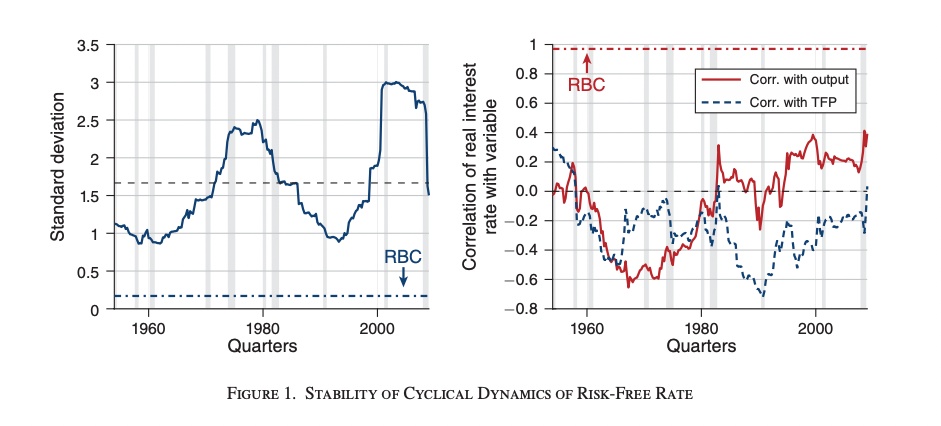
\includegraphics[scale=0.45]{figures/w_1}
\end{figure}
\end{frame}


\begin{frame}{Winberry 2021}
\begin{figure}
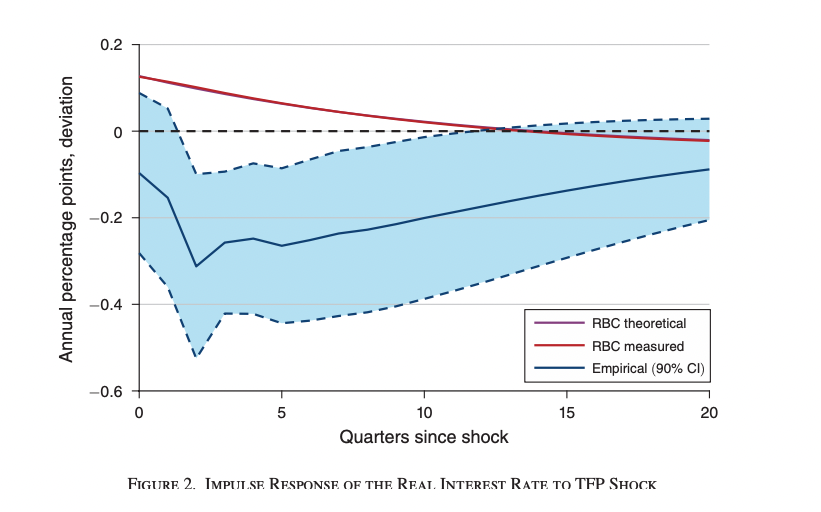
\includegraphics[scale=0.45]{figures/w_2}
\end{figure}
\end{frame}

\begin{frame}{Winberry 2021}
\begin{figure}
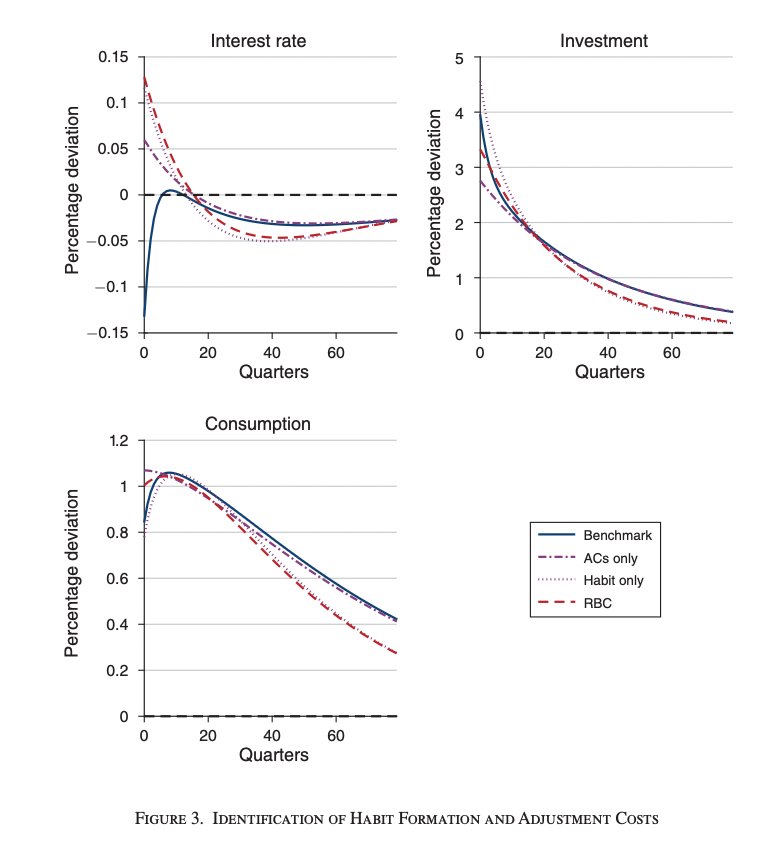
\includegraphics[scale=0.25]{figures/w_4}
\end{figure}
\end{frame}


\begin{frame}{Winberry 2021}
\begin{figure}
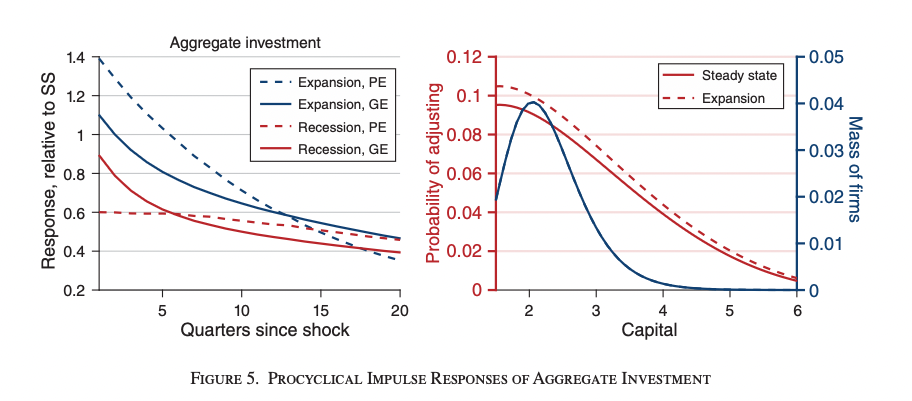
\includegraphics[scale=0.45]{figures/w_3}
\end{figure}
\end{frame}



\begin{frame}{How to tell models apart?}
\begin{itemize}
\item Koby and Wolf (2021) proposal: Use Zwick and Mahon (2017)
\item Semi-elasticity of investment to bonus depreciation reforms
\item Preview: Semi-Elasticity of investment in the data is consistent with Winberry (2021), not with Khan and Thomas (2008)
\end{itemize}
\end{frame}

\section{Zwick Mahon (2017)}

\begin{frame}{Bonus Depreciation}
\begin{itemize}
	\itemsep1em 
	\item Firms pay taxes on income net of business expenses
	\item Can fully expense wages, advertising, etc. immediately
	\item Investment gets expensed over time according to \\ tax depreciation schedules 
	\item Bonus depreciation accelerates this depreciation schedule
\end{itemize}
\end{frame}


\begin{frame}
\begin{figure}
	\centering
	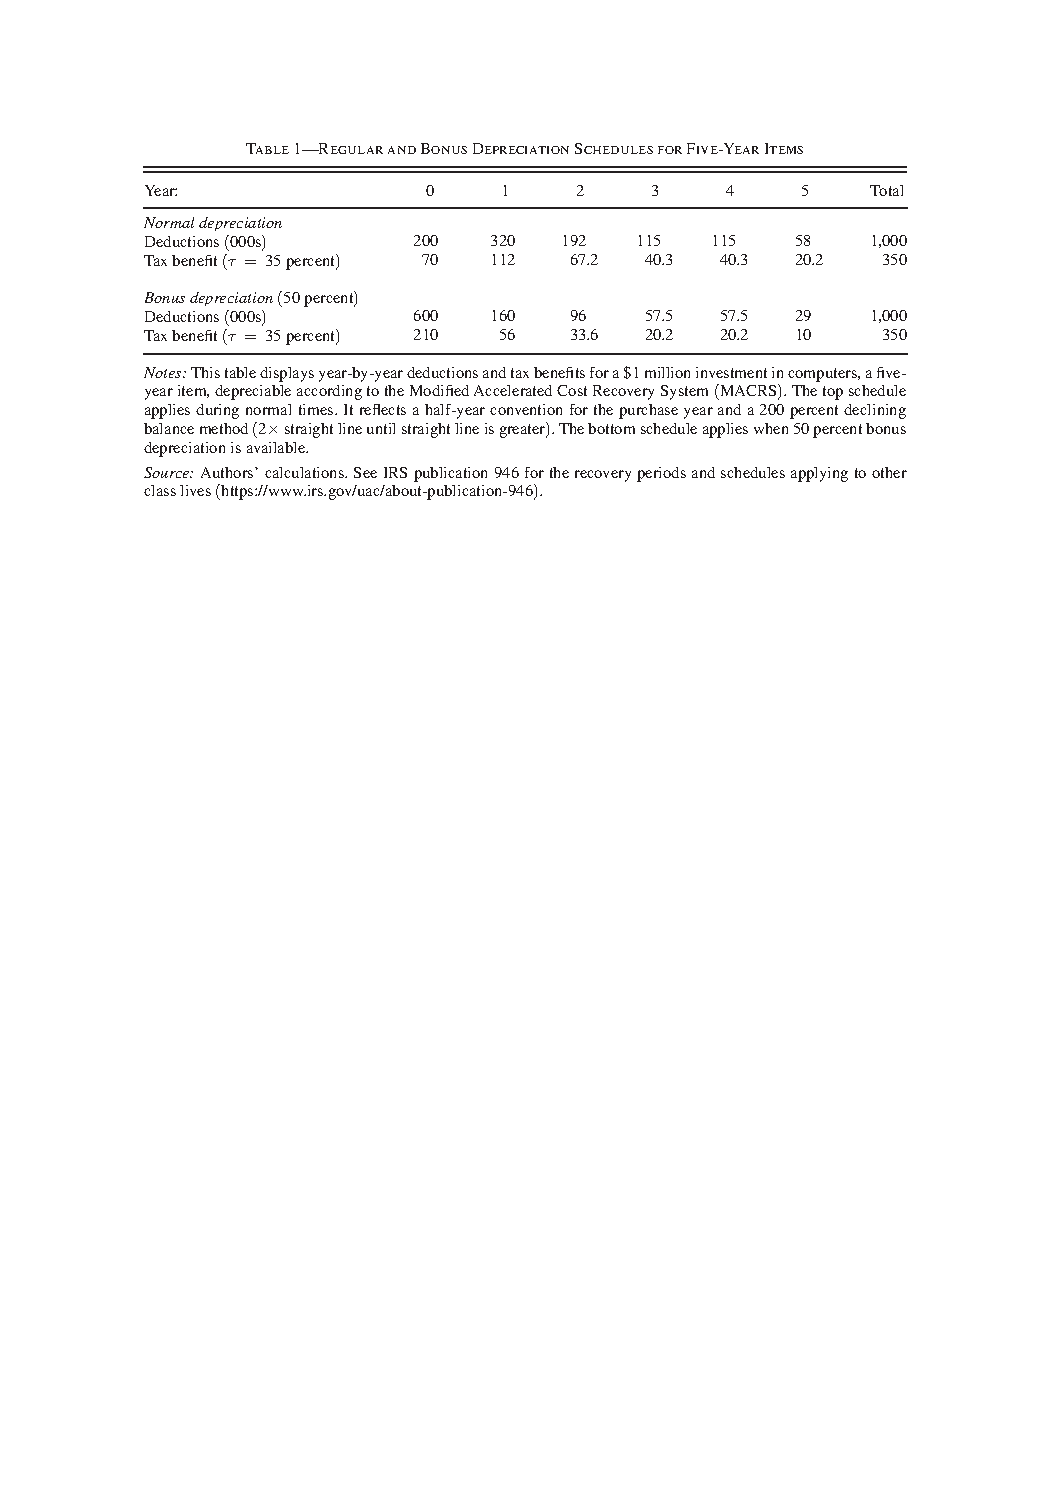
\includegraphics[width=0.65 \textwidth]{figures/ZwickMahon2017Table1.pdf}
\end{figure}
\vspace{-4mm}
{\scriptsize Source: Zwick-Mahon (2017)}
{\small 
\begin{itemize}
	\item Bonus depreciation allows firm to deduct a per dollar bonus of $\theta$ at the time of investment and the remaining $1-\theta$ according to regular schedule
	\item Table shows bonus depreciation of $\theta = 0.5$
\end{itemize} }
\end{frame}


\begin{frame}{Value of Bonus Depreciation}
Frictionless markets view:
\begin{itemize}
	\item Bonus depreciation only matters due to discounting
	\[ z^0 = D_0 + \sum_{t=1}^{T} \frac{1}{(1+r)^t} D_t \]
	\item $D_t$ allowable deduction in period $t$ per dollar of investment in period $0$
	\item $r$ risk-adjusted discount rate used by firm
	\item Without discounting $z_0 = 1$ (100\%), with discounting $z_0 < 1$
	\item Bonus raises $z_0$ by bringing deductions forward in time
	\[z = \theta + (1-\theta) z_0 \] 	
\end{itemize}
\end{frame}


\begin{frame}{Value of Bonus Depreciation}
\begin{itemize}
	\itemsep1em 
	\item Frictionless markets view:
	\begin{itemize}
		\item Value of bonus modest for short-lived investments
		\item E.g., with $r = 0.07$, bonus in Table 1 raised $z$ by 2\%
		\item Value of bonus greater for long-lived investments
	\end{itemize}
	\item With financial frictions, bonus may have large effect on investment
	\begin{itemize}
		\item Effect on current cash flow large (\$140,000 in Table 1) 
	\end{itemize}
\end{itemize}
\end{frame}


\begin{frame}{Zwick-Mahon (2017)}
\begin{itemize}
	\itemsep1em 
	\item Estimate the effect of bonus on investment
	\item Bonus occurs in recessions
	\begin{itemize}
		\item Correlated with other determinants of investment
	\end{itemize}
	\item Use difference-in-difference identification strategy
	\begin{itemize}
		\item Bonus more valuable for industries with longer lived investments
		\item Compare effect of bonus on industries with differing duration of investments 
	\end{itemize}
\end{itemize}
\end{frame}


\begin{frame}{Zwick-Mahon (2017): Policy Variable}
\begin{itemize}
	\itemsep1em 
	\item Main policy variable: $z_{N,t}$
	\begin{itemize}
		\item Where $N$ is a 4-digit NAICS industry
	\end{itemize}
	\item Compute baseline $z_N$ for pre-period (1993-2000)
	\begin{itemize}
		\item For each firm-year: weighted average of $z$ across duration categories using a 7\% discount rate
		\item $z_N$ computed as simple average of these firm-year $z$
	\end{itemize}
	\item In bonus years adjust $z_N$ for bonus
	\[z_{N,t} = \theta_t + (1-\theta_t)z_N \]  
\end{itemize}
\end{frame}


\begin{frame}{Zwick-Mahon (2017): Specification}
\begin{itemize}
	\item Baseline difference-in-difference specification:
	\[\log(I_{it}) = \alpha_i + \beta z_{N,t} + \gamma X_{it} + \delta_t + \epsilon_{it} \] \vspace{-15pt} 
	\begin{itemize}
		\item $\beta$ is coefficient of interest
		\item Industry fixed effects: Allow for average differences in industry investment
		\item Time fixed effects: Take out aggregate effects
	\end{itemize}
\end{itemize}
\end{frame}


\begin{frame}{Zwick-Mahon (2017): Identification}
\begin{itemize}
	\itemsep1em 
	\item Identifying assumption: \textbf{Parallel trends}
	\begin{itemize}
		\item Industries with long- and short-duration investment patterns would have evolved in parallel absent bonus
	\end{itemize}
	\item Threat to identification:
	\begin{itemize}
		\item Durable investment industries more resilient in downturns
	\end{itemize}
\end{itemize}
\end{frame}


\begin{frame}
\begin{figure}
	\centering
	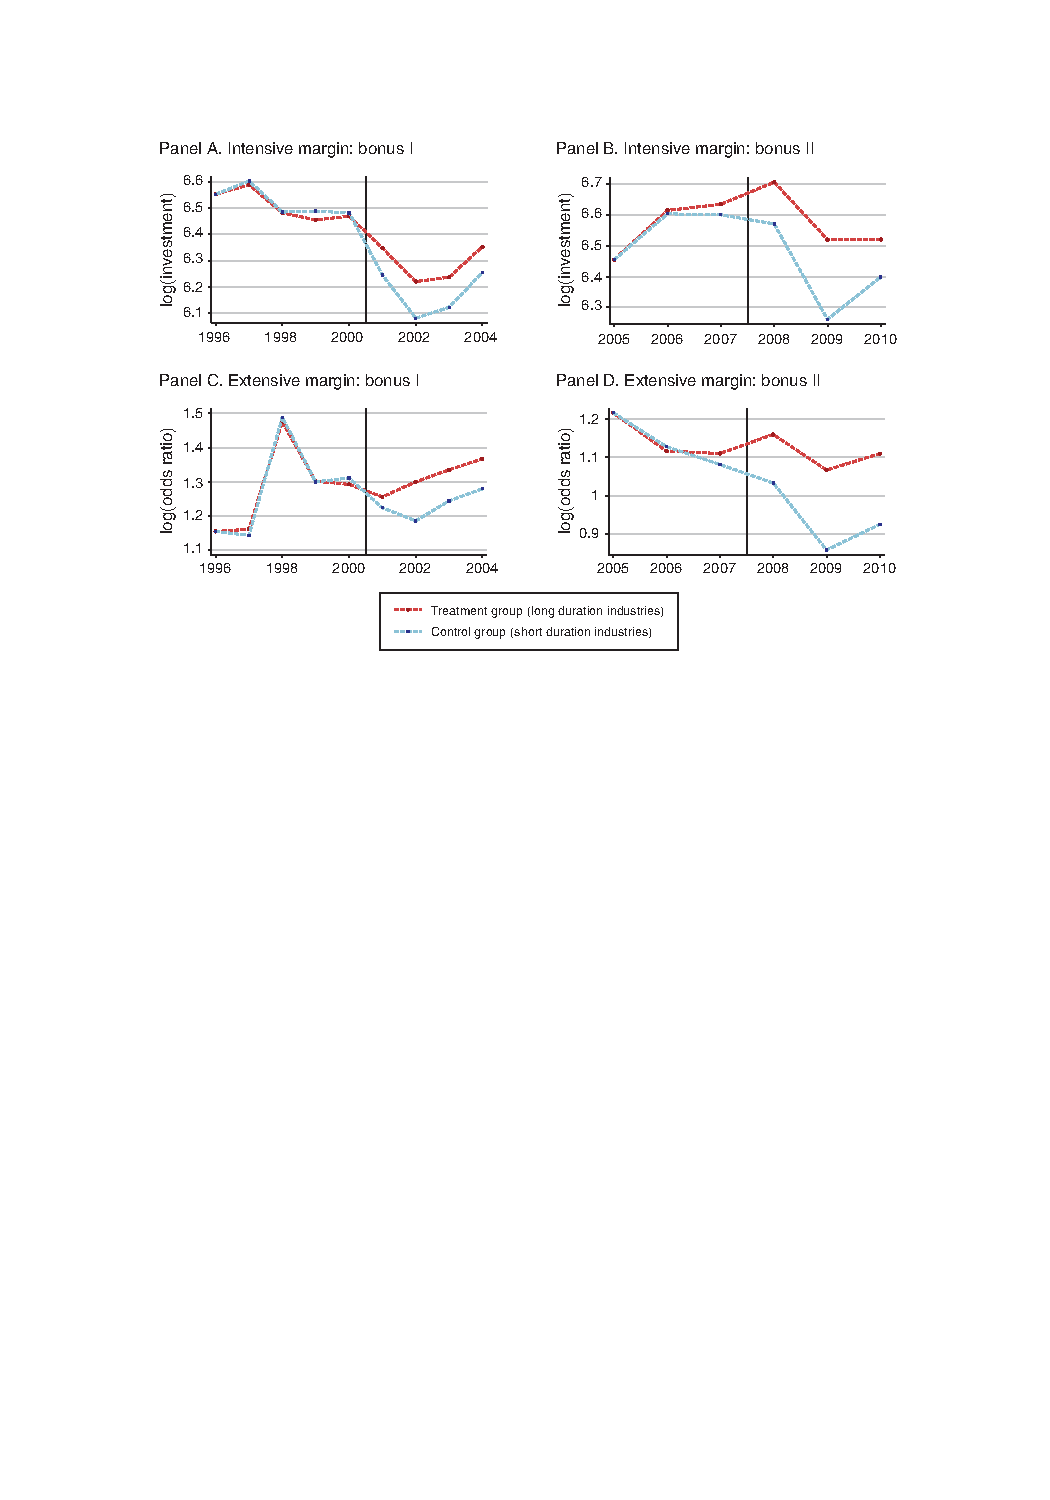
\includegraphics[height=0.85 \textheight]{figures/ZwickMahon2017Figure1.pdf}
\end{figure}
\vspace{-4mm}
{\scriptsize Source: Zwick-Mahon (2017)}
\end{frame}


\begin{frame}
\begin{figure}
	\centering
	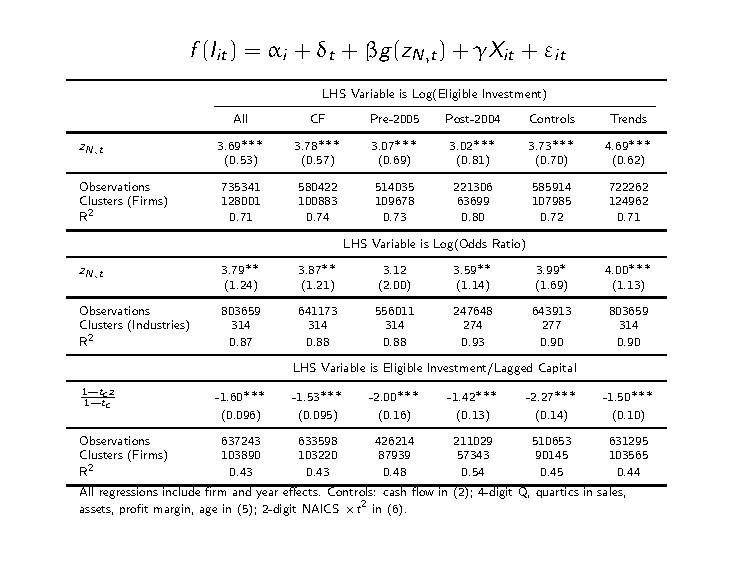
\includegraphics[height=0.9 \textheight]{figures/ZwickMahon2017Table3.pdf}
\end{figure}
\vspace{-4mm}
{\scriptsize Source: Zwick-Mahon (2017)}
\end{frame}


\begin{frame}{Zwick-Mahon (2017): Effects Are Large}
\begin{itemize}
	\itemsep1em 
	\item Average change in $z_{N,t}$: 
	\begin{itemize}
		\item Early episode: 4.8 cents
		\item Later episode: 7.8 cents
	\end{itemize}
	\item Average change in investment:
	\begin{itemize}
		\item Early episode: 17.7 log points (3.69 x 0.048 = 0.177)
		\item Later episode: 28.8 log points (3.69 x 0.078 = 0.288)	
	\end{itemize}
\end{itemize}
\end{frame}


\begin{frame}{Zwick-Mahon (2017): Effects Are Large}
\begin{itemize}
	\itemsep1em 
	\item In simple investment model:
	\begin{itemize}
		\item Elasticity of investment with respect to net of tax rate, $1-\tau z$, \\ equals price and interest elasticity
	\end{itemize}
	\[ \log (I_{it}) = \alpha + \beta \log(1-\tau z_{N,t}) + \epsilon_{it} \]
	\item Zwick-Mahon's regressor is $z_{N,t}$ not $\log(1-\tau z_{N,t})$
	\item Linear approximation:
	\[ \log(1-\tau z_{N,t}) =  \log(1-\tau z_{N}) - \frac{\tau}{1-\tau z_{N}} (z_{N,t} - z_N)  \] 
	\item Imply price and interest rate elasticities \\ of investment equal to
	\[- 3.69 \div \frac{\tau}{1-\tau z} \approx -7.2 \] 
\end{itemize}
\end{frame}

\section{Ottonello Winberry (2021)}

\begin{frame}{Motivation}
\begin{itemize}
\item Investment is the most cyclical component of aggregate demand
\item Investment Channel of Monetary Policy
\item What determines the strength of this effect?
\item Underlying notion of state-dependence
\end{itemize}
\end{frame}

\begin{frame}{Two Possibilities}
\begin{itemize}
\item Two possibilities on which firms respond more:
\begin{enumerate}
\item More constrained firms: Monetary policy expansions ease financial frictions. More constrained firms respond by more. Financial accelerator story
\item Less constrained firms: More constrained firms have steeper marginal cost curves, so they react by less to the same aggregate demand shock
\end{enumerate}
\item Ultimately an empirical question
\end{itemize}
\end{frame}

\begin{frame}{Specification}
\begin{itemize}
\item Basic specification
\[\Delta \log k_{j,t+1} = \alpha_j  = \alpha_j + \alpha_{st}  + \beta(x_{jt-1} - \mathbb{E}_j (x_{jt})) \epsilon^m_t + \Gamma' Z_{jt-1} + e_{jt}  \]
\item Where $\epsilon^m$ is determined using HFI
\[\epsilon^m_t = \tau(t) \times(ffr_{t+\Delta_+} - ffr_{t-\Delta_-})\]
\item Size of the window: -15 to +45 minutes
\end{itemize}
\end{frame}


\begin{frame}{Basic Result}
\begin{figure}
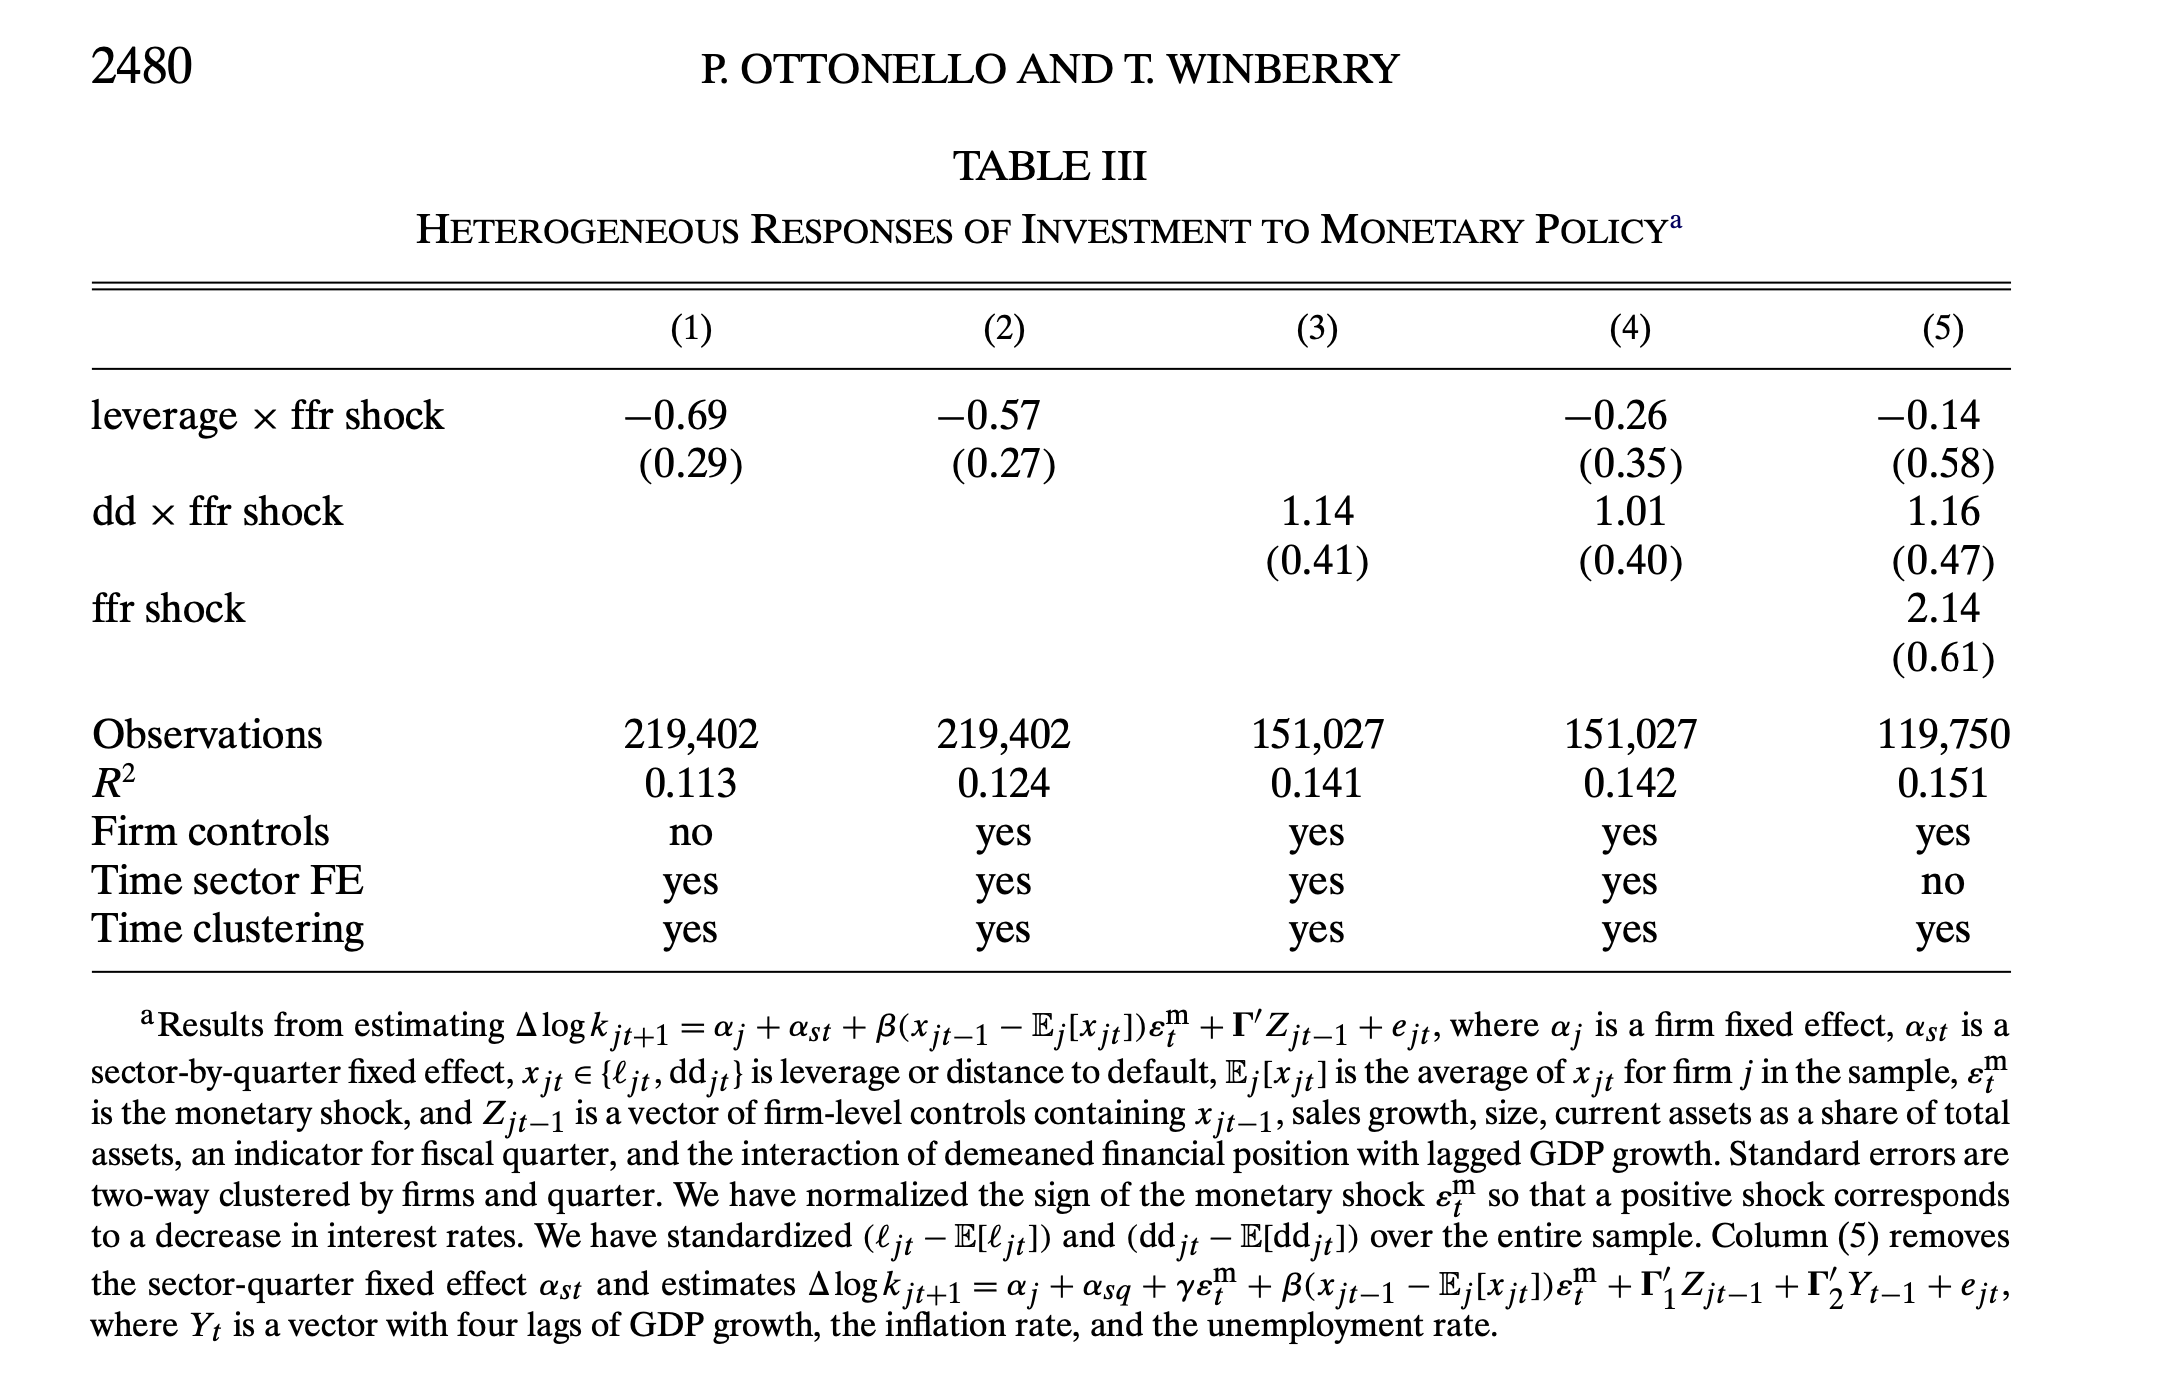
\includegraphics[scale=0.3]{figures/ow_1}
\end{figure}
\end{frame}


\begin{frame}{Dynamic Response}
\begin{figure}
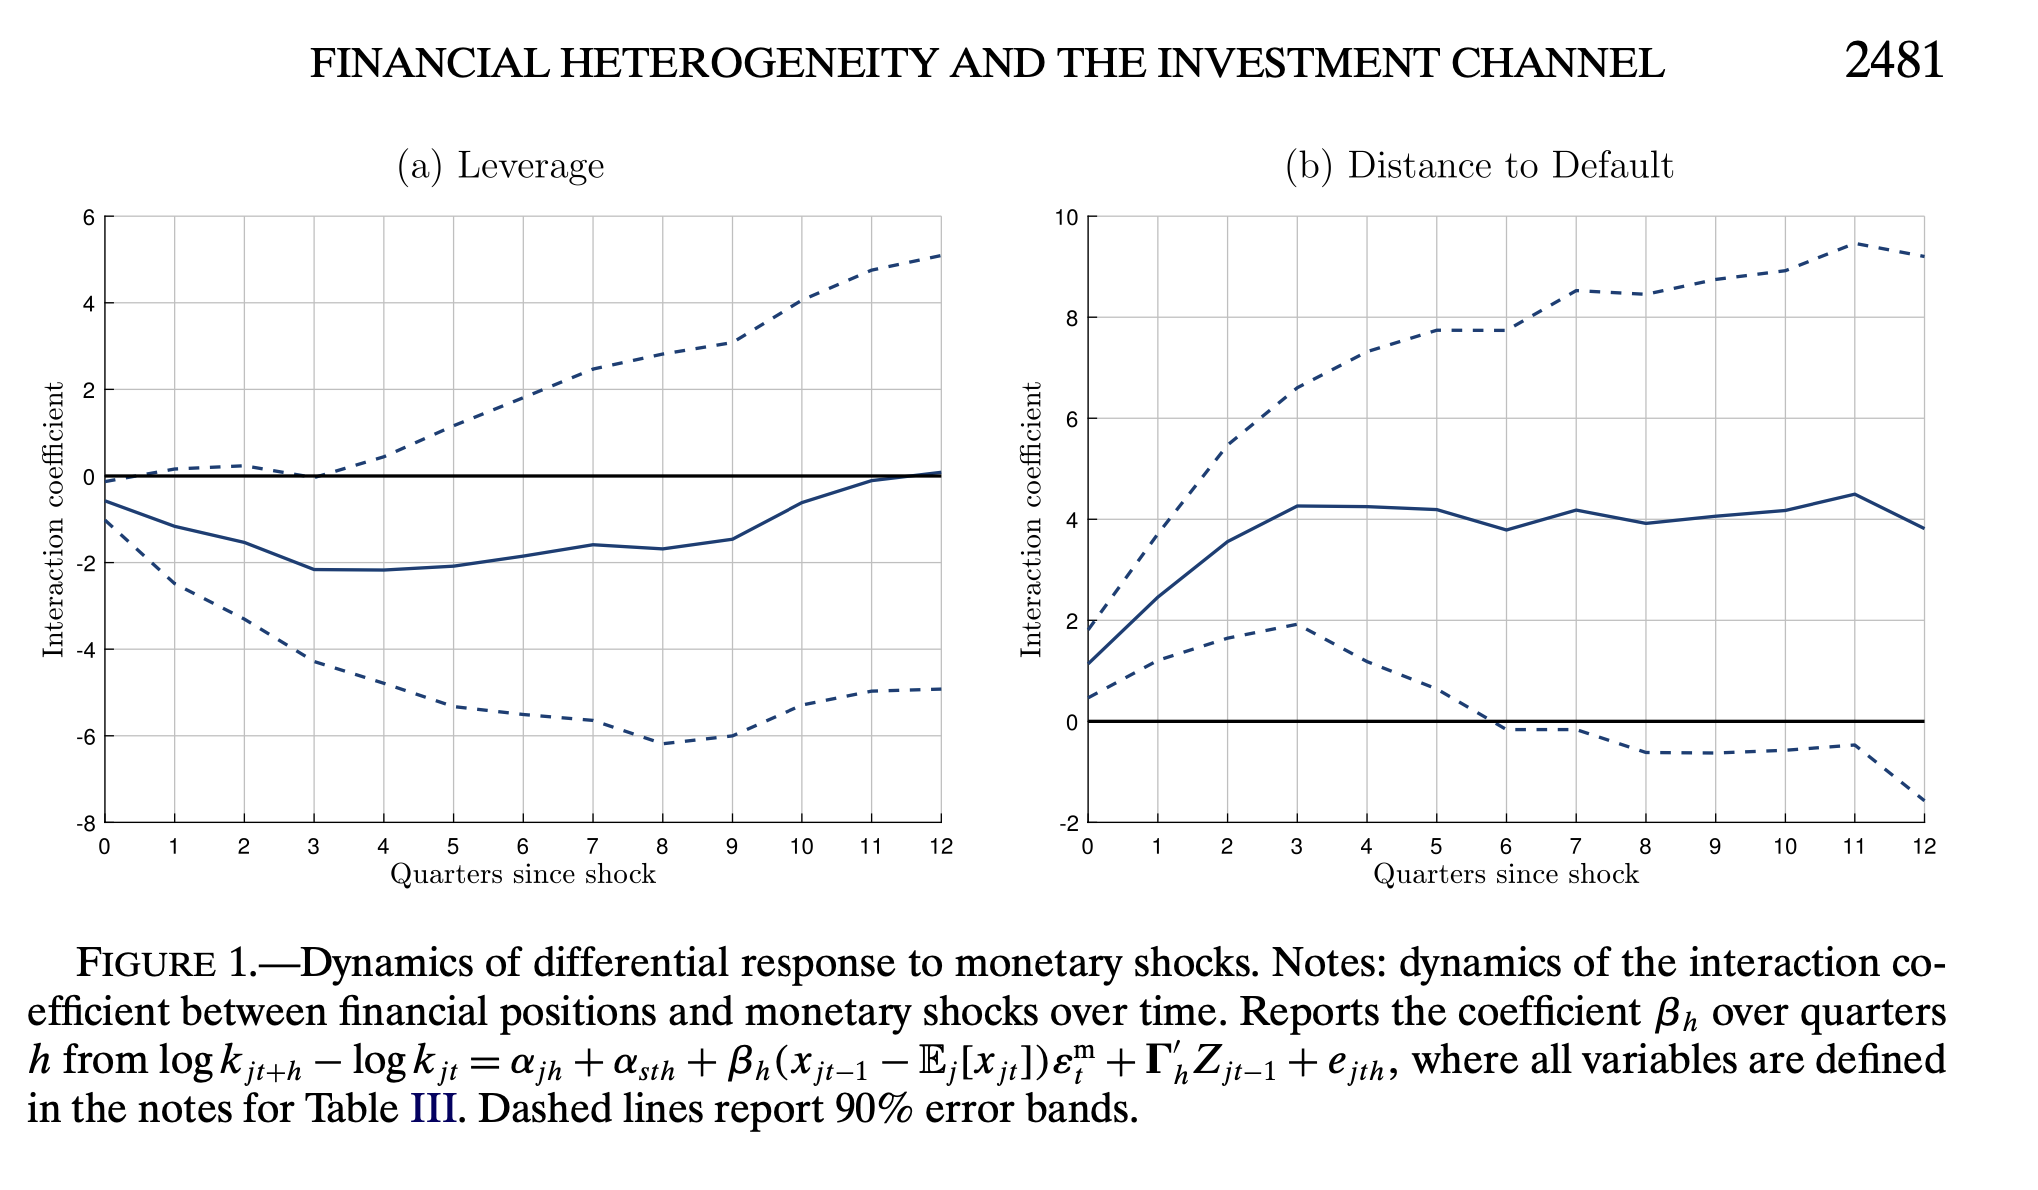
\includegraphics[scale=0.35]{figures/ow_2}
\end{figure}
\end{frame}


\begin{frame}{Model - Financial structure}
\begin{itemize}
\item No aggregate uncertainty
\item MIT shock later on
\item Firms can borrow in defaultable debt
\begin{itemize}
\item This is the optimal contract of Costly State Verification models (Townsend 1979)
\item Backbone of financial accelerator models (BGG 1999)
\end{itemize}
\item Retain earnings, not issue equity (think of infinite costs of equity issuance)
\item Without financial frictions need to keep track of only net worth, not $k$ and $b$ separately. Not possible with financial frictions
\item Economics: External finance premium/One unit of external finance is more costly
\end{itemize}
\end{frame}


\begin{frame}{Capital Producers}
\begin{itemize}
\item Capital producer sector
\item Relative price of investment $q$
\item q-theory FOC
\[q_t= \frac{1}{\Psi'(I_t/K_t)}\]
\end{itemize}
\end{frame}

\begin{frame}{Retailers - NK firms}
\begin{itemize}
\item Set prices subject to Rotemberg (1982) frictions
\item Relative price of retail goods $p$
\item Gives rise to a standard NK Phillips Curve
\end{itemize}
\end{frame}

\begin{frame}{Lenders}
\begin{itemize}
\item Intermediary, gets funds from the household, lends to firms
\item CSV block. Upon default (or verification) the lender gets $\alpha$ fraction of the market value of the firm stock
\item Price contracts at $\mathcal{Q}(z,k',b')$ to get zero profits (free entry in the background)
\end{itemize}
\end{frame}

\begin{frame}{Production Firms}
\begin{itemize}
\item DRS
\item exit shocks
\item Fixed costs of operation
\item Need a source of variation that suddenly brings firms closer to default
\item Capital quality shock
\textit{We view capital quality shocks as capturing unmodeled forces which reduce the value of the firm’s capital, such as frictions in the resale market, breakdown of machinery, or obsolescence.}
\item Effective units of capital $\omega k$	
\item Firms decide whether to default or not
\end{itemize}
\end{frame}

\begin{frame}{When to default}
\begin{itemize}
\item A firm receives a capital-quality shock $\omega$
\item The firm has some debt $b$ and the value of its capital goes down $\omega k$
\item Its net worth $n = \max_l p_t z (\omega k)^{\theta}l^{\nu} - w_t l + q_t (1-\delta) \omega k - b \frac{1}{\Pi_t} - \xi$ goes down
\item $\exists$ $\underline{n}$ such that the firm cannot respect the non-negativity on equity issuance
\[n - q_t k' + \mathcal{Q}(z,k',b')b' \geq 0\]
\end{itemize}
\end{frame}

\begin{frame}{Main Mechanism}
\begin{figure}
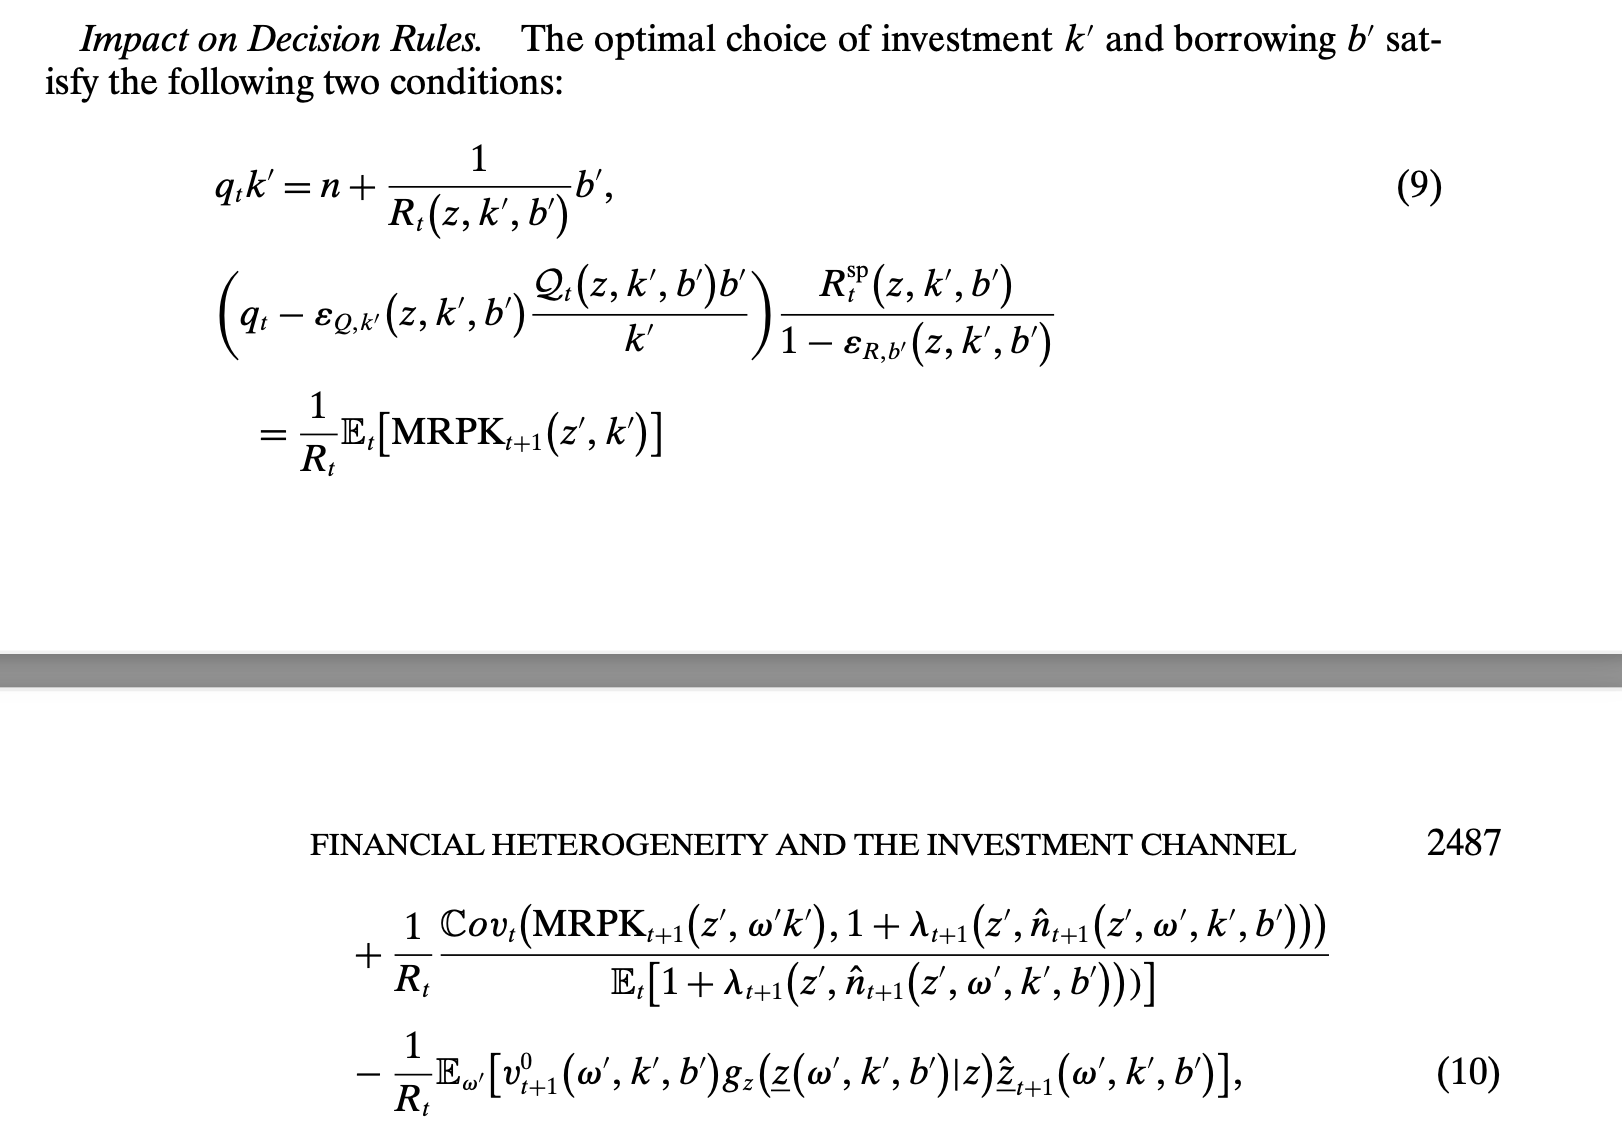
\includegraphics[scale=0.35]{figures/ow_6}
\end{figure}
\end{frame}


\begin{frame}{Intuition Main Mechanism}
\begin{figure}
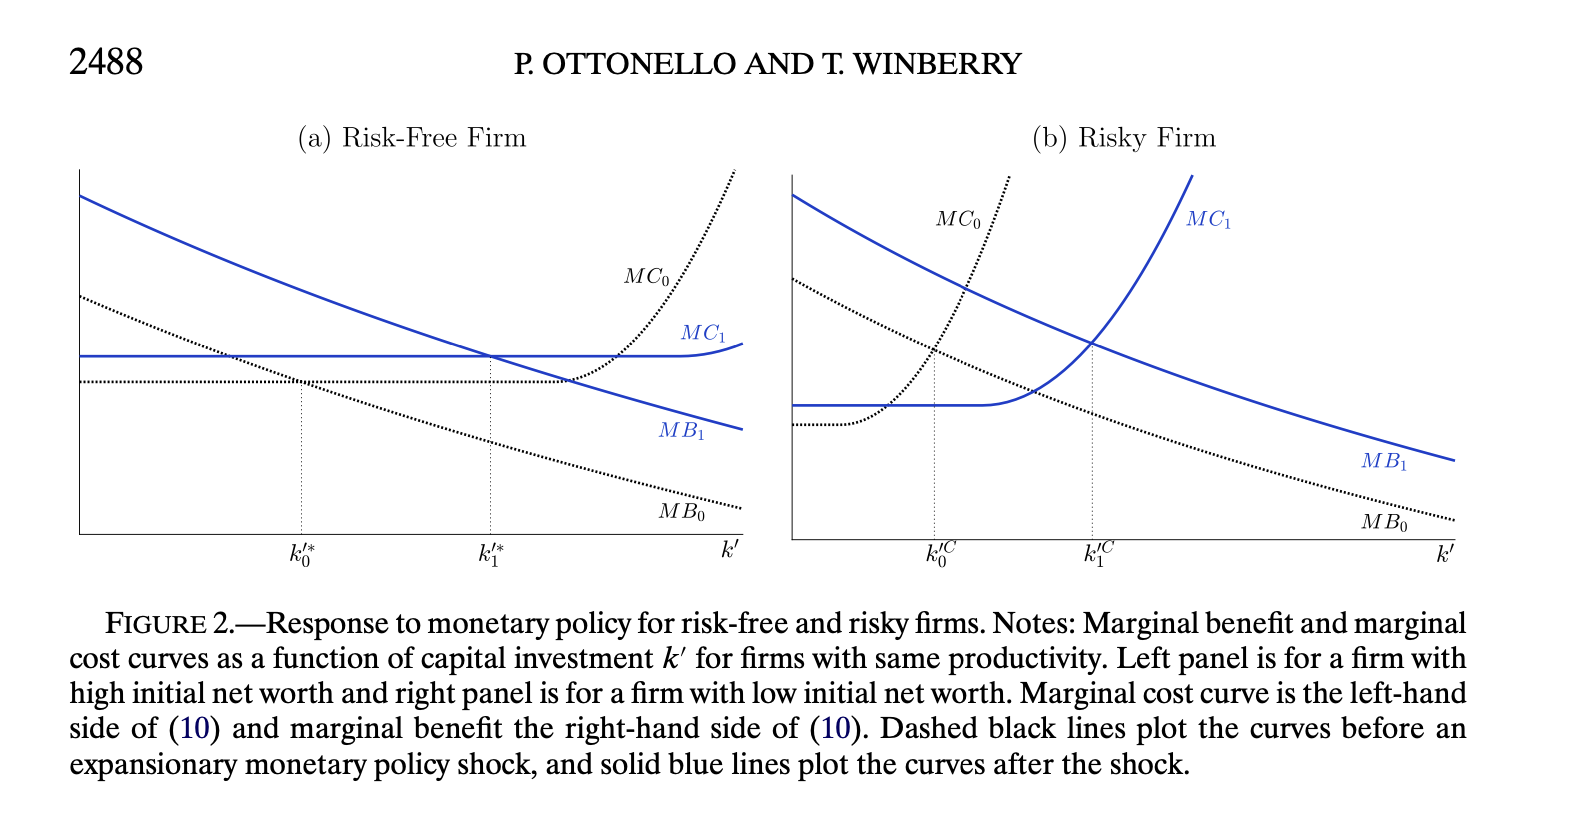
\includegraphics[scale=0.45]{figures/ow_7}
\end{figure}
\end{frame}

\begin{frame}{Intuition Main Mechanism}
\begin{figure}
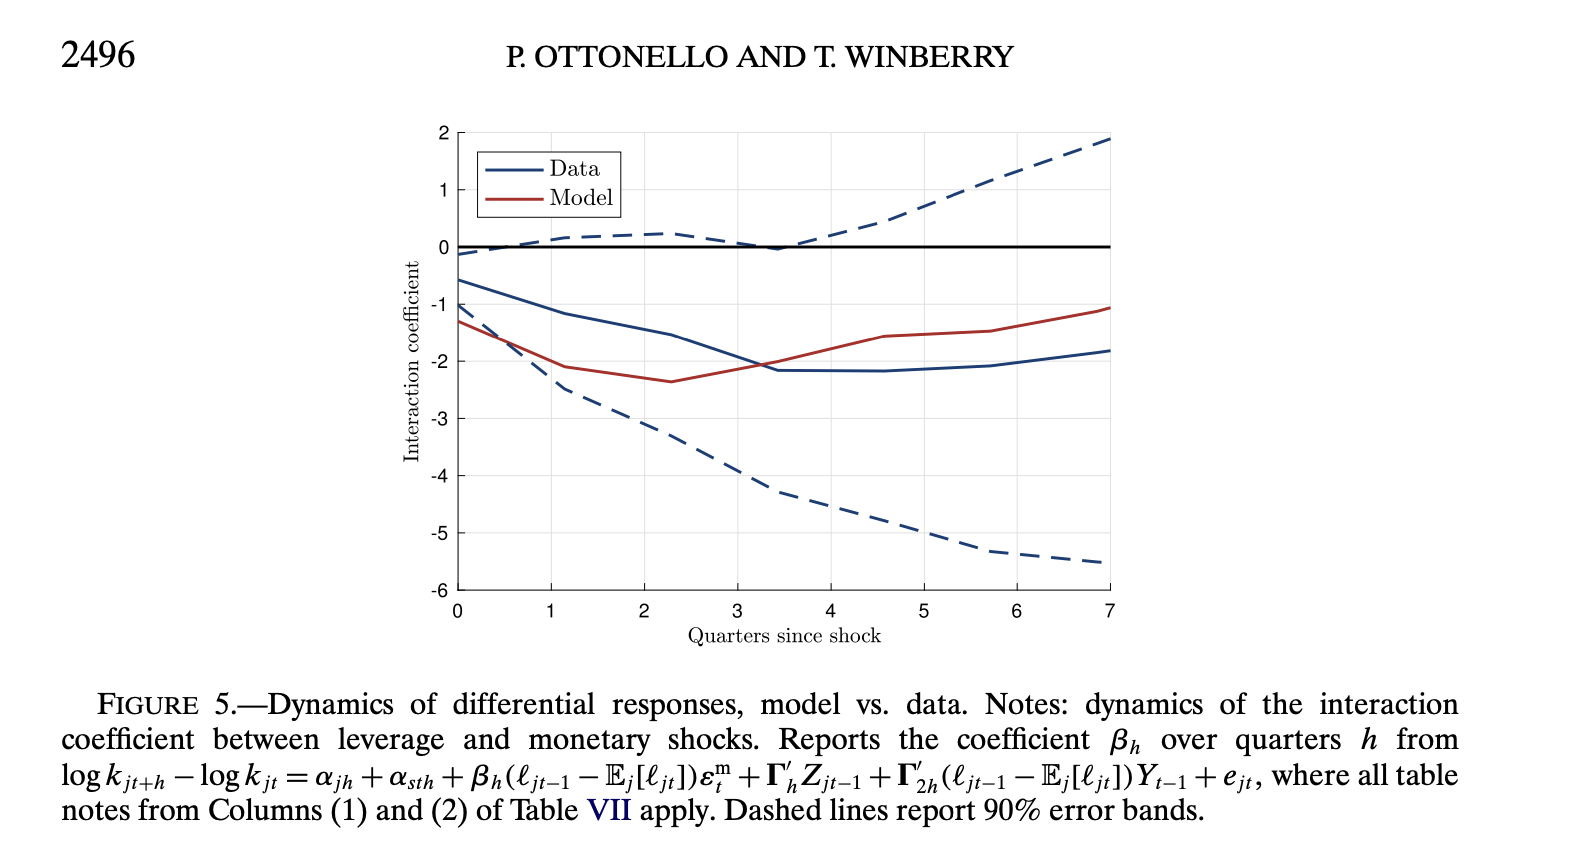
\includegraphics[scale=0.45]{figures/ow_3}
\end{figure}
\end{frame}


\begin{frame}{Intuition Main Mechanism}
\begin{figure}
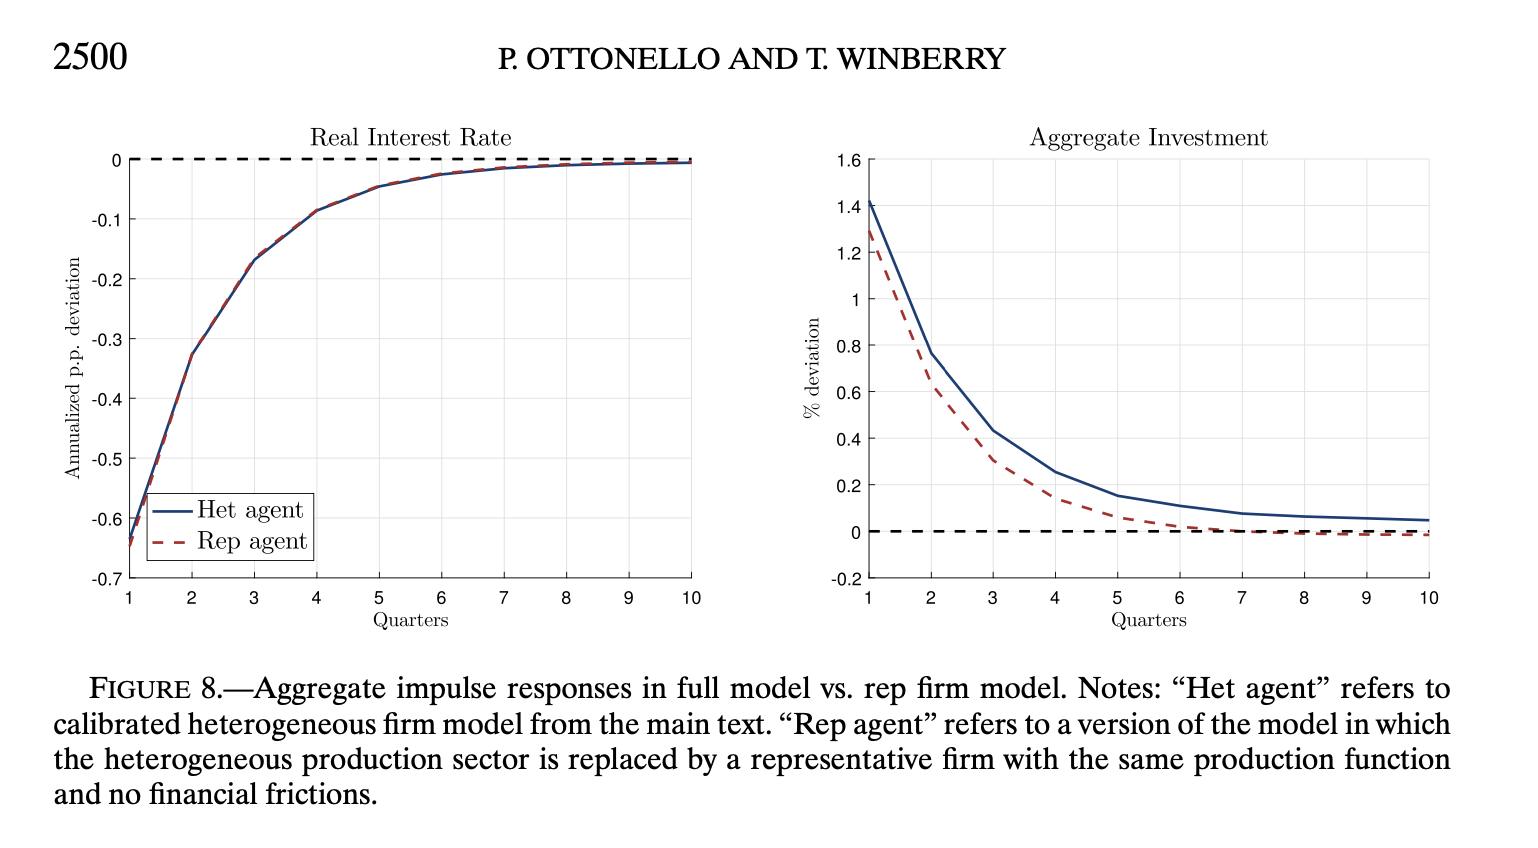
\includegraphics[scale=0.45]{figures/ow_4}
\end{figure}
\end{frame}


\begin{frame}{Intuition Main Mechanism}
\begin{figure}
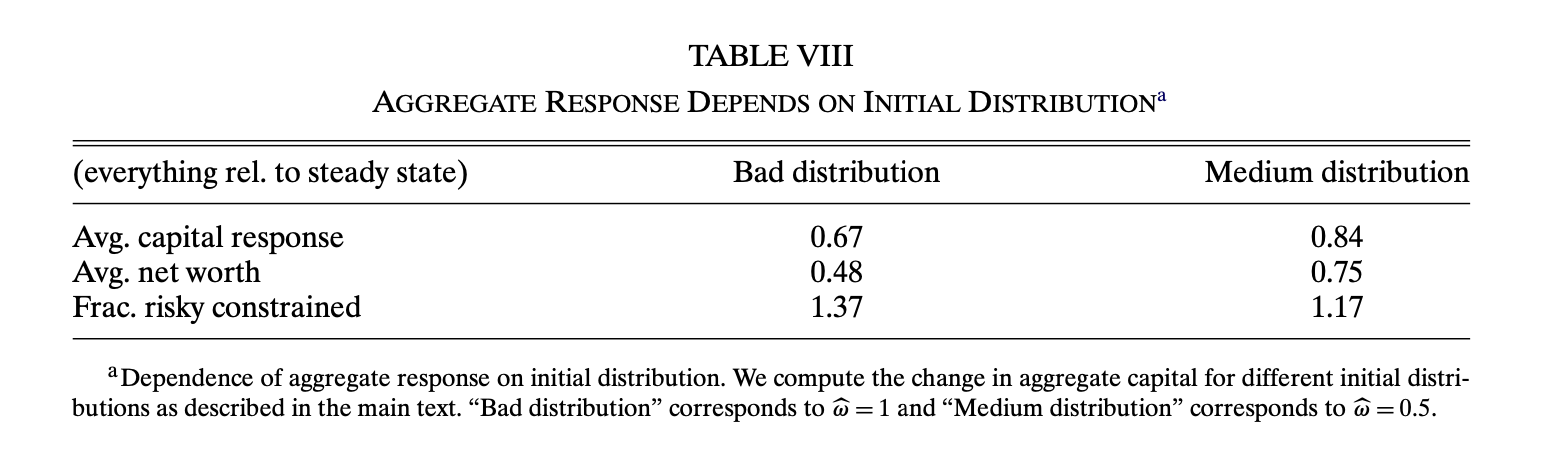
\includegraphics[scale=0.45]{figures/ow_5}
\end{figure}
\end{frame}


\end{document}